%  LaTeX support: latex@mdpi.com 

%=================================================================
\documentclass[micromachines,article,accept,pdftex,moreauthors]{Definitions/mdpi} 

%--------------------
% Class Options:
%--------------------
%----------
% journal
%----------

%---------
% article
%---------

%----------
% submit
%----------

%------------------
% moreauthors
%------------------
%---------
% pdftex
%---------

%=================================================================
% MDPI internal commands
\firstpage{1} 
\makeatletter 
\setcounter{page}{\@firstpage} 
\makeatother
\pubvolume{1}
\issuenum{1}
\articlenumber{0}
\pubyear{2022}
\copyrightyear{2022}
\externaleditor{Academic Editor: {Tiefeng Li}} % please add if has
\datereceived{23 December 2021} 
\dateaccepted{10 January 2022} 
\datepublished{} 

\hreflink{https://doi.org/} % If needed use \linebreak
%\doinum{}
%------------------------------------------------------------------

%=================================================================

\usepackage{graphics} % for pdf, bitmapped graphics files
\usepackage{subfigure}
\usepackage{amssymb}
\usepackage{amsbsy}

\usepackage[ruled,vlined]{algorithm2e}

%%% Coloring the comment as blue for the algorithm
\newcommand\mycommfont[1]{\footnotesize\ttfamily\textcolor{blue}{#1}}
\SetCommentSty{mycommfont}
\SetKwInput{KwInput}{Input}                % Set the Input
\SetKwInput{KwOutput}{Output}              % set the Output

\DeclareMathOperator{\atantwo}{atan2}
\DeclareMathOperator{\arctantwo}{arctan2}

%=================================================================
% Full title of the paper (Capitalized)
\Title{A Novel Distribution for Representation of 6D Pose Uncertainty}

% MDPI internal command: Title for citation in the left column
\TitleCitation{A Novel Distribution for Representation of 6D Pose Uncertainty}

% Author Orchid ID: enter ID or remove command
%\newcommand{\orcidauthorA}{0000-0000-0000-000X} % Add \orcidA{} behind the author's name
%\newcommand{\orcidauthorB}{0000-0000-0000-000X} % Add \orcidB{} behind the author's name

% Authors, for the paper (add full first names)
\Author{{Lei Zhang} %MDPI: Please carefully check the accuracy of names and affiliations.
 $^{1}$, Huiliang Shang $^{2}$ and Yandan Lin $^{3,}$*}
%\longauthorlist{yes}

% MDPI internal command: Authors, for metadata in PDF
\AuthorNames{Lei Zhang, Huiliang Shang and Yandan Lin}

% MDPI internal command: Authors, for citation in the left column
\AuthorCitation{{Zhang, L.}; {Shang, H.}; {Lin, Y.}
} %Lei Zhang: Please help to check this.

\address{%
$^{1}$ \quad Academy for Engineering and Technology, Fudan University, Shanghai {200433}, China; leizhang18@fudan.edu.cn\\
$^{2}$ \quad School of Information Science and Technology, Fudan University, Shanghai {200433}, China; shanghl@fudan.edu.cn\\
$^{3}$ \quad {Institute for Electric Light Sources, School of Information Science and Technology, Fudan University, Shanghai 200433, China}} %Lei Zhang: Added post code.


% Contact information of the corresponding author
\corres{Correspondence: ydlin@fudan.edu.cn}


% Abstract (Do not insert blank lines, i.e. \\) 
%Lei Zhang: I had updated the abstract, I marked as red font, please check and help to restore the black.
\abstract{The 6D Pose estimation is a crux in many applications, such as visual perception, autonomous navigation, and spacecraft motion. For robotic grasping, the cluttered and self-occlusion scenarios bring new challenges to the this field. Currently, society uses CNNs to solve this problem.{The CNN models will suffer high uncertainty caused by the environmental factors and the object itself.} These models usually maintain a Gaussian distribution, which is not suitable for { the underlying manifold structure of the pose}. {Many works decouple rotation from the translation and quantify rotational uncertainty. Only a few works pay attention to the uncertainty of the 6D pose.} This work proposes a distribution that can capture the uncertainty of the 6D pose parameterized by the dual quaternions, meanwhile, the proposed distribution takes the periodic nature of the underlying structure into account. The presented results include the normalization constant computation and parameter estimation techniques of the distribution. This work shows the benefits of the proposed distribution, which provides a more realistic explanation for the uncertainty in the 6D pose and eliminates the drawback inherited from the planar rigid motion.}

% Keywords
\keyword{probability theory; dual quaternion; pose uncertainty; lie group; Bingham distribution}
% , , , , pose estimation, L
% The fields PACS, MSC, and JEL may be left empty or commented out if not applicable
%\PACS{J0101}
%\MSC{}
%\JEL{}

%%%%%%%%%%%%%%%%%%%%%%%%%%%%%%%%%%%%%%%%%%

\begin{document}

%%%%%%%%%%%%%%%%%%%%%%%%%%%%%%%%%%%%%%%%%%%%%%%%%%%%%%%%%%%%%%%%%%%%%%%%%%%%%%%%%%%%

\section{Introduction} \label{sec:intro}

The Pose %MDPI: We have removed all the font color, please confirm. %Lei Zhang: Exactly, it should be removed
Estimation of rigid objects has a wide range of applications in today's life, such as {robot grasping} \cite{linRoboticGraspingMultiView2021}, aerospace applications, autonomous driving \cite{qidan2017rapid}, and so on.

Throughout history, pose estimation has played {a} vital role{, from Ceres's position predicting to navigation on the sea} (\cite{barfootStateEstimationRobotics2021}, {Introduction 1.1}).%MDPI: Please consider this suggested change. Similar highlights are same Meaning, please confirm all text %Lei Zhang: confirmed, I corrected 1.2 to 1.1.
{One day, } \textit{Captain cook} {sailing in the sea has lost his bearings. The ship moves on a wavy and wind sea. With the reasonable assumption, He estimates the optimal localization of the ship from the noisy measurements} (Figure~\ref{fig1}, top). %Lei Zhang: reworte the sentence, please help to check.

New challenges come to this field. The success of service robotics relies on well-perceiving an unfamiliar kitchen scenarios, such as bottles, dishes, and containers. Robot grasps under cluttered or limited lighting environments are becoming common in a rapidly growing warehouse automation industry \cite{zengRoboticPickandPlaceNovel2018}. Consequently, robots need to know the full 6D pose of objects to manipulate objects, which is difficult due to the uncertainty caused by environmental factors and sensing technologies. The intuition is to deploy expensive high-precision sensors to avoid such {uncertainty}. However, all sensors have limited precision, and measurements derived from actual sensors have associated uncertainty~\mbox{(\cite{barfootStateEstimationRobotics2021}, Introduction 1.2).} %Lei Zhang: no problem as your suggestion

 {The CNN \cite{krizhevsky2012imagenet} broke through in the ImageNet \cite{deng2009imagenet} challenge, motivating more and more works to embrace deep learning. However,}  most prior works in this area {failed} %Lei Zhang: since the things had happened already, I prefer use failed
 to take the weak information \cite{shamsfakhr2020gsr} and the {6D pose uncertainty} into account, and they only provide a single best guess for {each} %Lei Zhang: using each replace one
 object pose \cite{okornLearningOrientationDistributions2020, xiangPoseCNNConvolutionalNeural2018, wangDenseFusion6DObject2019}. The accurate metric of the model cannot handle unprepared situations, such as dim lighting. The uncertainty will rise with the increase in accuracy over time.

{The pose estimation of symmetric objects is currently the most challenging task} \cite{hodanEPOSEstimating6D2020}. %Lei Zhang: rewrote the sentence, remove the "due to CNNs failing to handle this"
{Existing multiple correct poses for the same visual appearance} \cite{manhardtExplainingAmbiguityObject2019}. {This issue also results} in lousy training performance since a network receives inconsistent loss signals. %Lei Zhang: reworte the sentence remove the redundant citation [8] \st{[8]}
Xiang et al. \cite{xiangPoseCNNConvolutionalNeural2018} design {an MSE loss function based on quaternions and regress the 3D rotation using the neural network.} {It reports better} performance for symmetric objects such as bowls. However, they do not take the underlying structure of the manifolds into consideration.

%Lei Zhang: rewrote the sentence
Deng et al. \cite{dengPoseRBPFRaoBlackwellizedParticle2019} {detect the object's position by a bounding box using a neural network. They assume the Gaussian position and approximate the observation likelihood to obtain the conditioning orientation density by a Rao--Blackwellized particle filter. The result is considerably robust in rotational uncertainty}. However, this approach is computationally expensive, and it is not clear which kind of distribution holds on the orientations. Furthermore, uncertain rotation axes need to be considered when underlying uncertainty is not axis aligned \cite{gilitschenskiDEEPORIENTATIONUNCERTAINTY2020}.

%Lei Zhang: rewrote here
Nonetheless, the {neural network} correctly assumes the underlying structure of the data is {robust}. Prokudin \cite{prokudinDeepDirectionalStatistics2018} exhibits {a good example dealing with periodic circular data}. The same loss will {emerge} when the predicted angle is equal to $1 \text{\textdegree}$ or $359 \text{\textdegree}$ with the ground truth angle {of} $0 \text{\textdegree}$. He {presents} a loss based on {the} directional setting and {assumes} the angle {obeys} the von Mises distribution. As a result, {the model} works {suitably} for the data {with the periodic nature}.

%Lei Zhang: rewrote here
{The} Gaussian {assumption} is commonly {embedded}, leading the neural network to fail to learn {the underlying manifold structure of the} 6D pose. {Holding the robust assumption of uncertainty is the foremost for 6D pose estimation}.

%Lei Zhang: rewrote here
Inevitably, {coupling or decoupling is the first consideration} when parametrizing the 6D pose. It is also related to {further modeling uncertainty}. 
%Lei Zhang: reorganized the sentences
Daniilidis \cite{daniilidisHandEyeCalibrationUsing1999} employs dual quaternion to parameterize the 6D pose for hand--eye calibration and establishes a linear homogeneous system, simultaneously solving rotation and translation. Goddard and Addi \cite{goddardPoseMotionEstimation1998} capture the correlation between rotation and translation for rigid motion tracking by dual quaternions.

%Lei Zhang: reorganized the sentences, update words marked by hl
Horn \cite{hornClosedformSolutionAbsolute1987} proposes the method that decouples the orientation from translation. Inspired by Horn, Srivatsan \cite{arun2018probabilistic} makes a linear assumption on the state of the {$SE(3)$} %Lei Zhang: I update the terms to mathematics representation, the following same.
elements by adopting dual quaternions. Li \cite{liGeometryDrivenStochasticModeling2019} explains the correlation between rotation and translation terms based on hyperspherical parallel transport and gives a {Bingham} distribution on the orientation decoupled from the translation. Manhardt \cite{manhardtExplainingAmbiguityObject2019} illustrates the rotation uncertainty caused by occlusion in the 6D pose estimation by employing {Bingham distribution}. However, it is still unknown how the Bingham distribution extends to {$SE(3)$} % Lei Zhang: to mathematics representation
space without variations.

%  The ICP \cite{beslMethodRegistration3D1992} is one of the state-of-the-art algorithms for point cloud registration that extends Horn’s idea. It iteratively estimates known point correspondence in two coordinate systems and performs least-squares optimization for the unknown point correspondence. Recently, Lin \cite{linRoboticGraspingMultiView2021} developed a technique by using multi-view scenes to decrease the initial error. %Lei Zhang: removed
% 

The work's most Bingham distribution of interest is motivated by Glover. The proposed BPA~\cite{gloverBinghamProcrusteanAlignment2013} algorithm  to recover the full poses from patches of local features of the 3D point cloud. This work is also based on the distribution over {$SE(2)$} %MDPI: Please check if italics/bold are required, The format in the equations, figures and text should be consistent, please check the full text.. % Lei Zhang: I checked all the terms of the SE(2) and the SE(3) , they should be in mathematics context.
 \cite{gilitschenskiNewProbabilityDistribution2014}, which uses the dual quaternions to parameterize $SE(2)$ elements, and a new distribution is proposed based on the parameterization results. The probability density function can naturally  capture the periodic nature of the underlying structure.


%%%%%%%%%%%%%%%%%%%%%%%%%%%%%%%%%%%%%%%%%%
%%%%%%%%%%%%%%%%%%%%%%%%%%%%%%%%%%%%%%%%%%
\subsection*{Main Contribution}

In this work {models} the uncertain 6D pose by extending the probability density function on {the $SE(2)$} %Lei Zhang: update to math representation.
to the {$SE(3)$}. This is achieved through parameterizing the 6D pose by dual quaternions. The work simplifies a future generalization to the 6D pose estimation of objects (Figure \ref{fig1}, bottom). The {proposed} distribution appears as a marginal distribution for the rotational part of the proposed model. We further discuss the relationship between orientation and position. To the best of the author's knowledge, there is no work exactly claimed for this.

This paper is organized as follows. We will compare several existing 6D parameterization techniques and select the most promising one in Section \ref{2}. In Section \ref{3}, we propose a new probability distribution on the 6D pose. The normalization constant and parameter estimation techniques will be discussed. Later, in Section \ref{4}, we use the proposed framework to represent the transformation of the 6D pose, and the algorithm that recovers the transformation from the samples of our proposed distribution will be presented. Lastly, the discussion and conclusions of this work are in Section \ref{5}.

%%%%%%%%%%%%%%%%%%%%%%%%%%%%%%%%%%%%%%%%%%

\begin{figure}[H]
\centering
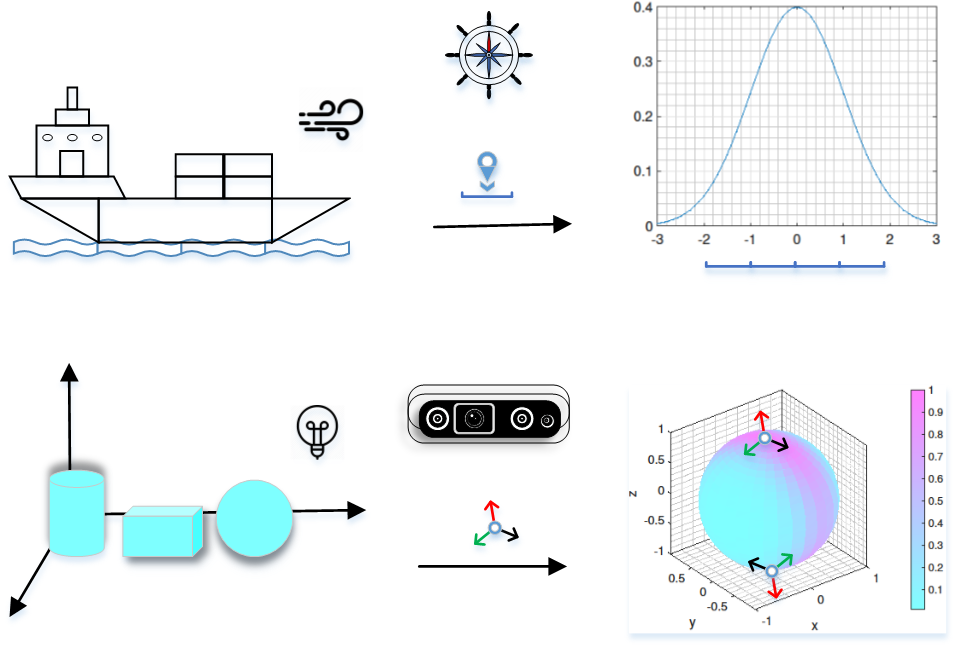
\includegraphics[width=10cm]{Definitions/figs/MODEL_UNCERTAINTY2.3.png}
\caption{{The analogy} %MDPI: It is suggested to change hyphen (-) to minus sign (–) in all figures. %Lei Zhang: I changed the color of the geometric objecs in the figure and centered the figure.
 to localize a ship moves on the sea. The position appears as the Gaussian distribution with noise measurements caused by the wind and waves. However, it is no longer suitable for the 6D pose uncertainty influenced by illumination and symmetric objects themselves. The result of the proposed distribution shows an antipodal symmetry for the 6D pose. \label{fig1}}
\end{figure}

%%%%%%%%%%%%%%%%%%%%%%%%%%%%%%%%%%%%%%%%%%

%%%%%%%%%%%%%%%%%%%%%%%%%%%%%%%%%%%%%%%%%%%%%%%%%%%%%%%%%%%%%%%%%%%%%%%%%%%%%%%%%%%%
\section{Preliminaries}\label{2}
There are several existing methods to parameterize $SE(3)$ elements, including orthonormal rotation matrices, Euler angles, Rodrigues vectors, quaternions, etc. For orthonormal rotation matrices, the compounding of two elements is much more complex (\cite{corkeRoboticsVisionControl2017}, {p. 45}). %Lei Zhang: I do no sure the p. 45 make sense, or should use pp. ? as your suggestion, I use p. instead.
Although Euler angles are invariant under transforms and easy to comprehend, there exist singularities \cite{jacksonPlanningAttitude2021}. Rodrigues vectors are complex to implement as a composition algorithm \cite{feiten20096d}.  {For parameterization of the 3D rotation, the quaternion is the best from the analog computation view \cite{stuelpnagelParametrizationThreeDimensionalRotation1964}. Still, it is also limited to representing rotation in a full 6D pose, and the translation must be dealt with separately}

The dual quaternions this work introduced takes both rotation and translation into consideration. It provides a closed-form solution for the composition of 6D poses, which is the analogy to the transform matrix in homogeneous coordinates \cite{feitenRigidMotionEstimation2013}.  {Kenwright \cite{kenwrightBeginnersGuideDualquaternions2012} finds that the transforms by the dual quaternion multiplication 10 percent faster compared to matrix multiplication on average. Nonetheless, Kavan et al. \cite{kavanSkinningDualQuaternions2007} present a practical example, and they utilize dual quaternions to solve the shortage of the linear blend skinning.}

{\textbf{Conventions}.} %MDPI: Is the bold necessary?. Lei Zhang: Yes, it functions as claim.
In this work, lower-case letters represent scalars, and matrices are represented by capital letters, vectors, and quaternions in bold. Quaternions are distinguished from dual quaternions by a caret, e.g., $\widetilde{\boldsymbol{q}}$ denotes a quaternion and $\widehat{\boldsymbol{q}}$ denotes a dual quaternion. Two quaternions $\widetilde{\boldsymbol{p}}$ and $\widetilde{\boldsymbol{q}}$ multiplication is denoted as  $\widetilde{\boldsymbol{p}} \odot \widetilde{\boldsymbol{q}}$, while the multiplication of the two dual quaternions is denoted as $\widehat{\boldsymbol{p}} \otimes \widehat{\boldsymbol{q}}$. The dot product and cross product of vectors $\boldsymbol{v}$ and $\boldsymbol{w}$ are denoted as $\langle{\boldsymbol{v},\boldsymbol{w}}\rangle$ and $\boldsymbol{v} \times \boldsymbol{w}$, respectively. Finally, we use $\mathbb{H}$ represent the skew-field of quaternions. With this in mind, consider the quaternions $\widetilde{\boldsymbol{q}} \in \mathbb{H}$. {The pose is synonymous with the 6D pose or transformation; the rotation is synonymous with orientation; the translation is synonymous with the position.} %Lei Zhang: add sentences here

%%%%%%%%%%%%%%%%%%%%%%%%%%%%%%%%%%%%%%%%%%
%%%%%%%%%%%%%%%%%%%%%%%%%%%%%%%%%%%%%%%%%%

\subsection{Quaternions} \label{2.1}
Similar to complex numbers, the sum of a real number and three complex numbers represent quaternions. The quaternion $\widetilde{\boldsymbol{q}} \in \mathbb{R}^4$ can be treated as a 4-tuple $(q_0, q_1, q_2, q_3) $. It can also be identified with the typical basis elements $i$, $j$, $k$ via the coefficients:
%%%%%%%BEGIN EQUATION%%%%%%%%%%
\begin{equation} \label{eq:1}
    \mathbb{H} ={\{} \widetilde{\boldsymbol{q}}{\ }|{\ }\widetilde{\boldsymbol{q}} = q_0 + q_1 i + q_2 j + q_3 k, {\ } {q_0,q_1,q_2,q_3 \in \mathbb{R}}  {\}}.
\end{equation}
%%%%%%%END EQUATION%%%%%%%%%%
The multiplication of the two quaternions $\widetilde{\boldsymbol{p}} = (p_0, \boldsymbol{p})$, $\widetilde{\boldsymbol{q}} = (q_0, \boldsymbol{q})$ is given by:
\begin{equation} \label{eq:2}
    \widetilde{\boldsymbol{p}} \odot \widetilde{\boldsymbol{q}}=p_{0} q_{0}- {\langle\boldsymbol{p}, \boldsymbol{q}\rangle} +q_{0} \boldsymbol{p}+p_{0} \boldsymbol{q}+\boldsymbol{p} \times \boldsymbol{q},
\end{equation}
\textls[-15]{where $p_0,q_0$ names the scalar part and $\boldsymbol{p},\boldsymbol{q}\in \mathbb{R}^3 $ is the vector part; note that the product is \mbox{not commutative.}}

Furthermore, linear operators \cite{fanDecentralizedRecursiveIdentification2017} $\boldsymbol{Q}_{p}^{+} \text{ and } \boldsymbol{Q}_{q}^{-}$ $\rightarrow \mathbb{R}^{4 \times 4}$ and associated with ($\ref{eq:2}$) can be also defined by matrix-vector form as:
%%%%%%%BEGIN EQUATION%%%%%%%%%%
\begin{equation} \label{eq:3}
    \widetilde{\boldsymbol{p}} \odot \widetilde{\boldsymbol{q}}=\boldsymbol{Q}_{p}^{+} \cdot \widetilde{\boldsymbol{q}} = \boldsymbol{Q}_{q}^{-} \cdot \widetilde{\boldsymbol{p}},
\end{equation}
%%%%%%%END EQUATION%%%%%%%%%%
with
%%%%%%%BEGIN EQUATION%%%%%%%%%%
\begin{align*}
    \boldsymbol{Q}_{p}^{+} = 
    \left[\begin{array}{cc}
        p_{0} & -\boldsymbol{p}^{T} \\
        \boldsymbol{p} & \boldsymbol{p}^{\times}+p_{0} \boldsymbol{I}_{3}
        \end{array}\right],\boldsymbol{Q}_{q}^{-} = 
    \left[\begin{array}{cc}
        q_{0} & -\boldsymbol{q}^{T} \\
        \boldsymbol{q} & -\boldsymbol{q}^{\times}+q_{0} \boldsymbol{I}_{3}
    \end{array}\right] .
\end{align*}
%%%%%%%END EQUATION%%%%%%%%%%
where $[\ ]^{\times}$ is the skew-symmetric matrix generated from the corresponding vector.

The canonical norm on $\mathbb {H}$ of quaternions is defined by $||\widetilde{\boldsymbol{q}}|| = \sqrt{\widetilde{\boldsymbol{q}} \odot \widetilde{\boldsymbol{q}}^{*}} = \sqrt{\widetilde{\boldsymbol{q}}^{*}
    \odot \widetilde{\boldsymbol{q}}} = 
    \sqrt{{q_0}^2 + {q_1}^2 + {q_2}^2 + {q_3}^2}.$

The conjugate of the quaternion is obtained by changing the sign of each element in the imaginary part: $\widetilde{\boldsymbol{q}}^{*} = (q_0, - \boldsymbol{q}) = (q_0, -q_1, -q_2, -q_3)$.

Last but not the least, the quaternion addition is simply the 4-tuple addition of quaternion representations:
$\widetilde{\boldsymbol{p}} + \widetilde{\boldsymbol{q}} = (p_0, \boldsymbol{p}) + (q_0, \boldsymbol{q}) = (p_0 + q_0, \boldsymbol{p} + \boldsymbol{q})$.

%%%%%%%%%%%%%%%%%%%%%%%%%%%%%%%%%%%%%%%%%%
%%%%%%%%%%%%%%%%%%%%%%%%%%%%%%%%%%%%%%%%%%

\subsection{Representation of 3D Rotation} \label{2.2}

Unit quaternions $\widetilde{\boldsymbol{q}}$ are quaternions with $||\widetilde{\boldsymbol{q}}|| = 1$ and commonly represent the rotations in 3D Euclid space.
The inverse of a unit quaternion is obtained by its conjugate form $\widetilde{\boldsymbol{q}}^{-1} = \widetilde{\boldsymbol{q}}^{*}$.

{The quaternion can represent the rotation around a 3D axis with a unit-length vector} $\boldsymbol{v}$ and the rotation angle $\theta \in [-\pi, \pi]$: %MDPI please check original meaning is maintained %Lei Zhang: Yes, this needs to be rewritten.
%%%%%%%BEGIN EQUATION%%%%%%%%%%
\begin{equation} \label{eq:4}
\widetilde{\boldsymbol{q}} = cos({\frac{\theta}{2}}) + \boldsymbol{v}sin({\frac{\theta}{2}}).
\end{equation}
%%%%%%%END EQUATION%%%%%%%%%%

A point $\boldsymbol{p} = (p_1, p_2, p_3) \in \mathbb{R}^3$ is denoted as the purely imaginary quaternion without real part $\widetilde{\boldsymbol{p}} = {p_1}i + {p_2}j + {p_3}k$. From ($\ref{eq:4}$), the rotated point $\widetilde{\boldsymbol{p}}_{rot}$ is obtained as \cite{feiten20096d}: 
%%%%%%%BEGIN EQUATION%%%%%%%%%%
\begin{align*}
    \widetilde{\boldsymbol{p}}_{rot} = \widetilde{\boldsymbol{q}} \odot \widetilde{\boldsymbol{p}} \odot
    \widetilde{\boldsymbol{q}}^{*}.
\end{align*}
%%%%%%%END EQUATION%%%%%%%%%%
In addition, $\widetilde{\boldsymbol{q}}$ and $-\widetilde{\boldsymbol{q}}$ represent the same rotation due to the \textit{antipodal} property on the hypersphere $\boldsymbol{S}^3$, so the set $\boldsymbol{U}$ of unit quaternion is a double coverage of the $SO(3)$ of the 3D rotations.

%%%%%%%%%%%%%%%%%%%%%%%%%%%%%%%%%%%%%%%%%%
%%%%%%%%%%%%%%%%%%%%%%%%%%%%%%%%%%%%%%%%%%

\subsection{Dual Quaternions} \label{2.3}
The dual theory is helpful when understanding the concept of dual quaternions. A dual number combines  the non-dual part $a_1$, and the dual part $b_1$ is represented as $a_1 + \epsilon b_1,$ where $a_1, b_1\in \mathbb{R}$. The $\epsilon$ is the dual unit; note that $\epsilon \neq 0$, $\epsilon^2 = 0$. The multiplication of two dual numbers is given as $(a_1 + \epsilon b_1)(a_2 + \epsilon b_2 ) = a_1a_2 + \epsilon(a_1b_2 + a_2b_1).$

Dual quaternions ($\widehat{\boldsymbol{x}} \in \mathbb{H}_D$) are quaternions equivalent to dual numbers, i.e., replacing real numbers $a_1, b_1$ with quaternions $\widetilde{\boldsymbol{p}}$ and $\widetilde{\boldsymbol{q}}$. Thus, a dual quaternion is given as follows:
%%%%%%%BEGIN EQUATION%%%%%%%%%%
\begin{equation} \label{eq:5}
    \mathbb{H}_D = \{ \widehat{\boldsymbol{x}} {\ }| {\ } \widehat{\boldsymbol{x}} = \widetilde{\boldsymbol{p}} + \epsilon
    \widetilde{\boldsymbol{q}}, \quad
    \widetilde{\boldsymbol{p}}, \widetilde{\boldsymbol{q}} \in \mathbb{H} \}.
\end{equation}
%%%%%%%END EQUATION%%%%%%%%%%

The multiply operation of two dual quaternions is similar to dual numbers. As two dual quaternions $\widehat{\boldsymbol{x}}_1 = \widetilde{\boldsymbol{p}}_1 + \epsilon \widetilde{\boldsymbol{q}}_1$ and  $ \widehat{\boldsymbol{x}}_2 = \widetilde{\boldsymbol{p}}_2 + \epsilon \widetilde{\boldsymbol{q}}_2$ ($\widehat{\boldsymbol{x}}_1, \widehat{\boldsymbol{x}}_2 \in \mathbb{H}_D$), the product of the two is:
%%%%%%%BEGIN EQUATION%%%%%%%%%%
\begin{equation} \label{eq:6}
\widehat{\boldsymbol{x}}_{1} \otimes \widehat{\boldsymbol{x}}_{2}=\widetilde{\boldsymbol{p}}_{1} \odot \widetilde{\boldsymbol{p}}_{2}+\epsilon\left(\widetilde{\boldsymbol{p}}_{1} \odot \widetilde{\boldsymbol{q}}_{2}+\widetilde{\boldsymbol{p}}_{2} \odot \widetilde{\boldsymbol{q}}_{1}\right).
\end{equation}
%%%%%%%END EQUATION%%%%%%%%%%
Note that the product is non-commutative.

The dual quaternions apply the same strategy utilized by quaternions, linear operators: $(\cdot)^{+}$ and $(\cdot)^{-} \in \mathbb{R}^{8 \times 8}$ can be defined for dual quaternions by:
%%%%%%%BEGIN EQUATION%%%%%%%%%%
\begin{equation*}
\widehat{\boldsymbol{x}}_{1} \otimes \widehat{\boldsymbol{x}}_{2} = \boldsymbol{Q}_{{x}_1}^{+} \cdot \widehat{{x}}_{2} = \boldsymbol{Q}_{{x}_2}^{-} \cdot \widehat{{x}}_{1},
\end{equation*}
with
\begin{equation*}
\boldsymbol{Q}_{{x}_1}^{+} = 
    \left[\begin{array}{cc}
        \boldsymbol{Q}_{p_1}^{+} & \boldsymbol{O} \\
        \boldsymbol{Q}_{q_1}^{+} & \boldsymbol{Q}_{p_1}^{+}
    \end{array}\right],
\boldsymbol{Q}_{{x}_2}^{-} = 
    \left[\begin{array}{cc}
        \boldsymbol{Q}_{p_2}^{-} & \boldsymbol{O} \\
        \boldsymbol{Q}_{q_2}^{-} & \boldsymbol{Q}_{p_2}^{-}
        \end{array}\right].
\end{equation*}
%%%%%%%END EQUATION%%%%%%%%%%

Dual quaternions have three conjugates \cite{fanDecentralizedRecursiveIdentification2017}: 1) $\widehat{\boldsymbol{x}}^{1*} = \widetilde{\boldsymbol{p}} - \epsilon \widetilde{\boldsymbol{q}}$, 2) $\widehat{\boldsymbol{x}}^{2*} = \widetilde{\boldsymbol{p}}^{*} + \epsilon \widetilde{\boldsymbol{q}}^{*}$, and 3) $\widehat{\boldsymbol{x}}^{3*} = \widetilde{\boldsymbol{p}}^{*} - \epsilon \widetilde{\boldsymbol{q}}^{*}$. A dual quaternion $\widehat{\boldsymbol{x}}$ is a unit if $\widehat{\boldsymbol{x}} \otimes \widehat{\boldsymbol{x}}^{2*} = 1$.

The norm of a dual quaternion in ($\ref{eq:5}$) is denoted as $||\widehat{\boldsymbol{x}}|| = \sqrt{\widehat{\boldsymbol{x}} \otimes \widehat{\boldsymbol{x}}^{2*}} = \sqrt{\widehat{\boldsymbol{x}}^{2*} \otimes \widehat{\boldsymbol{x}}}$, which expands to:
%%%%%%%BEGIN EQUATION%%%%%%%%%%
\begin{align*}
    ||\widehat{\boldsymbol{x}}|| = \sqrt{\widehat{\boldsymbol{x}} \otimes \widehat{\boldsymbol{x}}^{2*}} = ||\boldsymbol{p}|| + \epsilon{\frac{ \langle \boldsymbol{p},\boldsymbol{q} \rangle}{||\boldsymbol{p}||}}.
\end{align*}
%%%%%%%END EQUATION%%%%%%%%%%
The unit dual quaternions have the norm that equals one. A dual quaternion satisfies the unit dual quaternion if and only if the non-dual part $||\boldsymbol{p}||$ equals one and the dot product of two parts $\langle\boldsymbol{p},\boldsymbol{q}\rangle$ equals zero. This property helps to understand the relationship between the two parts of the dual quaternion. Especially, a unit quaternion is a unit dual quaternion when the dual part is zero.

%%%%%%%%%%%%%%%%%%%%%%%%%%%%%%%%%%%%%%%%%%
%%%%%%%%%%%%%%%%%%%%%%%%%%%%%%%%%%%%%%%%%%

\subsection{Representation of 6D Pose}  \label{2.4}
The 6D pose composes a 3D rotation part represented by a unit quaternion $\widetilde{\boldsymbol{q}}_r = [q_0, q_1, q_2, q_3]$ in the form of ($\ref{eq:4}$) and a 3D translation part $\boldsymbol{t} \in \mathbb{R}^3$. A unit dual quaternion representing the 6D pose is defined by the following equation:
\begin{equation} \label{eq:7}
    \widehat{\boldsymbol{x}}_{d} = 
    \widetilde{\boldsymbol{q}}_{r} + \epsilon \widetilde{\boldsymbol{q}}_{d},
\end{equation}
where $\widetilde{\boldsymbol{q}}_{d}$ for translation $\boldsymbol{t}$ is defined by:
%%%%%%%BEGIN EQUATION%%%%%%%%%%
\begin{equation} \label{eq:8}
    \widetilde{\boldsymbol{q}}_{d} = \frac{
    \widetilde{\boldsymbol{t}} \odot
    \widetilde{\boldsymbol{q}}_{r}}{2},
\end{equation}
%%%%%%%END EQUATION%%%%%%%%%%
where $\widetilde{\boldsymbol{t}}$ is represented by a purely imaginary translation quaternion with zero real parts.

We introduce the Hamilton operators $\boldsymbol{H}^{+},{\ } \boldsymbol{H}^{-}$ to replace the linear operators defined above. The term Hamilton operator, which is borrowed from Akyar \cite{akyarDualQuaternionsSpatial2008}, is not commonly used, at least in the robotics literature, but it seems appropriate here:
%%%%%%%BEGIN EQUATION%%%%%%%%%%
\begin{equation*}
    \boldsymbol{H}_{r}^{-} = 
        \left[\begin{array}{cc}
        q_{0} & -\boldsymbol{q}^{T} \\
        \boldsymbol{q} & -\boldsymbol{q}^{\times}+q_{0} \boldsymbol{I}_{3}
    \end{array}\right] =
    \begin{bmatrix}
    {q_0} &  {-q_1} &  {-q_2} &  {-q_3} \\
    {q_q} &  {q_0} & {q_3} &  {-q_2} \\
    {q_2} &  {-q_3} &  {q_0} & {q_1} \\
    {q_3} & {q_2} &  {-q_1} &  {q_0} 
    \end{bmatrix}
\end{equation*}
%%%%%%%END EQUATION%%%%%%%%%%
so that 
\begin{equation} \label{eq:9}
    \widetilde{\boldsymbol{q}}_{d} = \frac{1}{2} \boldsymbol{H}_{t}^{+}\widetilde{\boldsymbol{q}}_{r}
    = \frac{1}{2} \boldsymbol{H}_{r}^{-}\widetilde{\boldsymbol{t}}.
\end{equation}
where $\boldsymbol{H}_{t}^{+}$ is a $\mathbb{R}^{4 \times 4}$ skew-symmetric matrix generated from translation vector $\boldsymbol{t}$.

A point $p=(x,y,z)^T \in \mathbb{R}^3$, we can be embedded in skew-field $\mathbb{H}_D$ by using a dual quaternion $\widehat{\boldsymbol{x}}_{d}$ in ($\ref{eq:7}$). The transformation can be mathematically described as:
%%%%%%%BEGIN EQUATION%%%%%%%%%%
\begin{equation} \label{eq:10}
    \widehat{\boldsymbol{x}}_{d} \otimes
    \widehat{\boldsymbol{p}}_{d} \otimes
    \widehat{\boldsymbol{x}}_{d}^{3*}
\end{equation}
%%%%%%%END EQUATION%%%%%%%%%%
Consistent with the unit quaternion in rotations, the dual quaternions $\widehat{\boldsymbol{x}}_{d}$ and $-\widehat{\boldsymbol{x}}_{d}$ represent the \mbox{same pose.}

%%%%%%%%%%%%%%%%%%%%%%%%%%%%%%%%%%%%%%%%%%%%%%%%%%%%%%%%%%%%%%%%%%%%%%%%%%%%%%%%%%%%

\section{Methods} \label{3}

%%%%%%%%%%%%%%%%%%%%%%%%%%%%%%%%%%%%%%%%%%
%%%%%%%%%%%%%%%%%%%%%%%%%%%%%%%%%%%%%%%%%%
\subsection{Base Element}\label{3.1}
Consider the fact that the unit dual quaternions ${\boldsymbol{\widehat{d}_q}}$ and ${-\boldsymbol{\widehat{d}_q}}$ in the form of ($\ref{eq:5}$) represent the same pose. Furthermore, the underlying structure of the periodic nature of the 6D pose is no longer linear. Hence, a distribution that can characterize the non-linear structure antipodal symmetric property is required. Consequently, we can tackle multiple, conflicting hypotheses that naturally arise in ambiguous situations.

A Bingham distribution \cite{binghamAntipodallySymmetricDistribution1974} is exactly a distribution on a unit hypersphere $\boldsymbol{S}^{d-1}$. The property of hte most interest is the antipodal symmetric, where $dF(-\boldsymbol{x}) = dF(\boldsymbol{x})$ (i.e., opposite points on $\boldsymbol{S}^{d-1}$ have equal probability). It commonly represents uncertainty on 3D rotations, denoted as $SO(3)$ mathematically, by the unit quaternion form \cite{antoneRobustCameraPose2001}, but not on the 6D pose. \\

\noindent\textbf{Definition 1.} \textit{Let a random vector on the hypersphere} $\boldsymbol{S}^{d-1} = \{ 
{\boldsymbol{x}} \in \mathbb{R}^{d}: ||{\boldsymbol{x}}|| = 1 \} \subset \mathbb{R}^{d}$ \textit{be the unit hypersphere in} $\mathbb{R}^{d}$. \textit{The probability density function(p.d.f)}
%%%%%%%BEGIN EQUATION%%%%%%%%%%
\begin{align*}
    f {\ :\ } \boldsymbol{S}^{d-1} \rightarrow \mathbb{R}
\end{align*}
%%%%%%%END EQUATION%%%%%%%%%%
\textit{of a Bingham distribution is given by:}
%%%%%%%BEGIN EQUATION%%%%%%%%%%
\begin{align*}
    f({\boldsymbol{x}}) = {\frac{1}{N}} \cdot \text{exp}({{\boldsymbol{x}}^{T}{V}\boldsymbol{\Lambda}\boldsymbol{V}^{T}{{\boldsymbol{x}}}})
\end{align*}
%%%%%%%END EQUATION%%%%%%%%%%
\textit{where} $\boldsymbol{V} \in \mathbb{R}^{d{\times}d}$ \textit{is an orthogonal matrix} ($\boldsymbol{V}\boldsymbol{V}^{T}=\boldsymbol{V}^{T}\boldsymbol{V}={\boldsymbol{I}}_{d{\times}d}$)
$ \textit{, describing the orientation, } \boldsymbol{\Lambda} = \text{diag}({\lambda_1}, \dots, \lambda_{d-1},\textit{0}) \in \mathbb{R}^{d \times d}$ with ${\lambda_1} \leq \dots \leq {\lambda_{d-1}} \leq 0$ \textit{as the concentration matrix, and $N$ as a corresponding normalization constant.}

\vspace{6pt}%{}

For the representation of small uncertainty, Bingham is almost near the Gaussian distribution, and for the large {uncertainty}, the Gaussian is worse (or even quite poor) than the Bingham \mbox{distribution \cite{kurzRecursiveEstimationOrientation2013}.} %Lei Zhang: replace all uncertainties by uncertainty.

For those who are familiar with multivariate Gaussian, the parameter matrices $\boldsymbol{V}$ and $\boldsymbol{\Lambda}$ can be derived via the eigendecomposition of a symmetric matrix $\boldsymbol{C}$ in subsequent {Section \ref{3.2}} (which is denoted as the inverse covariance matrix $\boldsymbol{\Sigma^{-1}}$ in multivariate Gaussian distribution).

%%%%%%%%%%%%%%%%%%%%%%%%%%%%%%%%%%%%%%%%%%
%%%%%%%%%%%%%%%%%%%%%%%%%%%%%%%%%%%%%%%%%%

\subsection{A New Distribution Model}\label{3.2}

For a quite intuitive interpretation, we decompose a unit dual quaternion $\widehat{\boldsymbol{x}}$ into  $(\boldsymbol{x}_{r}, \boldsymbol{x}_{d})$ in vector form. Thus, a joint probability density over the non-dual part, and the dual part can be denoted as the following Lemma 2.\\

\noindent\textbf{Lemma 2.} \textit{A random vector} $\boldsymbol{x} = (\boldsymbol{x}_{r}, \boldsymbol{x}_{d}) {\ }\in \mathbf{S}^{3} \times \mathbb{R}^4 $ \textit{is distributed to the proposed distribution, and the p.d.f is:}\\
%%%%%%%BEGIN EQUATION%%%%%%%%%%
\begin{align*}
    f(\boldsymbol{x}_{r}, \boldsymbol{x}_{d}) = {N(\boldsymbol{C})}^{-1} \cdot
    \text{exp}\left({
    {\begin{pmatrix} \boldsymbol{x}_{r} \\ \boldsymbol{x}_{d} \end{pmatrix}}^T
    \boldsymbol{C} 
    {\begin{pmatrix} \boldsymbol{x}_{r} \\ \boldsymbol{x}_{d} \end{pmatrix}}
    }\right),
\end{align*}
%%%%%%%END EQUATION%%%%%%%%%%
\textit{where} $\boldsymbol{x}_{r} \in \mathbf{S}^3$ \textit{and} $\boldsymbol{x}_{d} \in \mathbb{R}^4$, \textit{symmetric and positive definite} $\boldsymbol{C} \in \mathbb{R}^{8 \times 8}$,  \textit{and a normalization constant} $N(\boldsymbol{C})$.

\vspace{6pt}%{}

It is always possible to break a joint density into the product of two factors. We can work out the details for the joint case by employing the \textit{Schur complement}. First, let $\boldsymbol{C}$ in Lemma 2 be denoted as:
%%%%%%%BEGIN EQUATION%%%%%%%%%%
\begin{align*}
    \boldsymbol{C} = \begin{pmatrix}
    {\boldsymbol{C}_{11}} & {\boldsymbol{C}_{12}} \\
    {\boldsymbol{C}_{21}} & {\boldsymbol{C}_{22}}
    \end{pmatrix}
\end{align*}
%%%%%%%END EQUATION%%%%%%%%%%

with $\boldsymbol{C}_{ij} \in \mathbb{R}^{4 \times 4}$; note that $\boldsymbol{C}_{21}=\boldsymbol{C}_{12}^T$, according to the settings \cite{gilitschenskiNewProbabilityDistribution2014}, $\boldsymbol{C}_{11}$ needs to be symmetric, $\boldsymbol{C}_{12}$ may be arbitrary, and $\boldsymbol{C}_{22}$ has to be symmetric negative definite to ensure the antipodal symmetry, which we will further discuss in {Section \ref{sec:nc}}.\\

\noindent\textbf{Lemma 3.} \textit{The proposed probability density function can be rewritten as:}
%%%%%%%BEGIN EQUATION%%%%%%%%%%
\begin{align*}
    f(\boldsymbol{x}_{r},\boldsymbol{x}_{d})
    = N(\boldsymbol{C})^{-1} & \cdot  
    \text{exp}(\boldsymbol{x}_{r}^{T} \boldsymbol{A}_{1} \boldsymbol{x}_{r} \\
    & + {(\boldsymbol{x}_{d}-\boldsymbol{A}_2\boldsymbol{x}_{r})^{T} \boldsymbol{C}_{22} (\boldsymbol{x}_{d}-\boldsymbol{A}_2\boldsymbol{x}_{r})})
\end{align*}
%%%%%%%END EQUATION%%%%%%%%%%
\textit{where} $\boldsymbol{A}_{1} = \boldsymbol{C}_{11} - \boldsymbol{C}_{12}\boldsymbol{C}_{22}^{-1} \boldsymbol{C}_{21}$, $\boldsymbol{A}_{2} = -\boldsymbol{C}_{22}^{-1}\boldsymbol{C}_{21}$.

\textit{A proof is given in Appendix~\ref{append1}}.\\

From {Lemma 3}, the rotation part of the dual quaternion evidently appears as a Bingham distribution, which can be derived by marginalizing out the corresponding conditional distribution of the dual part.

Since the dual part, $\boldsymbol{x}_{d}$, combines the rotation and translation by a Hamilton product, a canonical way to describe dependencies between the position and the orientation of a dual quaternion is still unknown \cite{gilitschenskiNewProbabilityDistribution2014}. 

From (\ref{eq:9}), the dual part given the non-dual part $f(\boldsymbol{x}_{d} | \boldsymbol{x}_{r})$ can be treated as a multivariate Gaussian distribution $\mathcal{N}(\boldsymbol{A}_2\boldsymbol{x}_r, -\frac{\boldsymbol{C}_{22}^{-1}}{2})$. Thus, the joint density function from Lemma 3 can be rewritten as:
%%%%%%%BEGIN EQUATION%%%%%%%%%%
\begin{align*}
    f(\boldsymbol{x}_{r},\boldsymbol{x}_{d}) & = f(\boldsymbol{x}_{r})f(\boldsymbol{x}_{d}|\boldsymbol{x}_{r})
    \\ 
    & = {{N_{\mathcal{B}}}(\boldsymbol{A}_1)}^{-1} \cdot  \text{exp}\left(\boldsymbol{x}_{r}^{T} \boldsymbol{A}_{1} \boldsymbol{x}_{r}\right) \cdot \\
    & {\qquad} {N_{\mathcal{G}}}^{-1}  \cdot \text{exp}\left(
    {(\boldsymbol{x}_{d}-\boldsymbol{A}_2\boldsymbol{x}_{r})^{T} \boldsymbol{C}_{22} (\boldsymbol{x}_{d}-\boldsymbol{A}_2\boldsymbol{x}_{r})}
    \right).
\end{align*}
%%%%%%%END EQUATION%%%%%%%%%%
\textit{where} $\boldsymbol{A}_{1} = \boldsymbol{C}_{11} - \boldsymbol{C}_{12}\boldsymbol{C}_{22}^{-1} \boldsymbol{C}_{21}$, $\boldsymbol{A}_{2} = -\boldsymbol{C}_{22}^{-1}\boldsymbol{C}_{21}$.

%%%%%%%%%%%%%%%%%%%%%%%%%%%%%%%%%%%%%%%%%%
%%%%%%%%%%%%%%%%%%%%%%%%%%%%%%%%%%%%%%%%%%

\subsection{Normliazation Constant} \label{3.3}
The Bingham distribution is flexible for 3D rotation represented by the unit quaternion on the hypersphere $\mathbf{S}^{3}$. Although it represents {uncertainty}, %Lei Zhang: replace all uncertainties by uncertainty.
it is still not well propagated in the computer vision and robotics communities because the computation of the normalization constant is complex. The normalization constant, $F$, in the Bingham distribution is not closed form, which means the normalization constant, $F$, only has the numerical solution. However, several techniques can overcome this difficulty, such as caching techniques \cite{gloverMonteCarloPose2011} and saddlepoint approximations. It is still an area of active research \cite{gilitschenskiDEEPORIENTATIONUNCERTAINTY2020}.

Fortunately, the computational burden is alleviated by the method adapted from \cite{gilitschenskiNewProbabilityDistribution2014}. The normalization constant is written as follows according to the discussion:
%%%%%%%BEGIN EQUATION%%%%%%%%%%
\begin{align*}
N(\boldsymbol{C}) = & {{N_{\mathcal{B}}}(\boldsymbol{A}_1)} \cdot N_{\mathcal{G}} = \frac{2 \pi \sqrt{\operatorname{det}\left(-\frac{1}{2} \boldsymbol{C}_{22}^{-1}\right)}}{F\left(\boldsymbol{A}_1\right)},
\end{align*}
%%%%%%%END EQUATION%%%%%%%%%%
where $\boldsymbol{A}_1 = \boldsymbol{C}_{11}-\boldsymbol{C}_{12} \boldsymbol{C}_{22}^{-1} \boldsymbol{C}_{21}$.

\textls[-5]{Furthermore, this work calculates ${{N_{\mathcal{B}}}(\boldsymbol{A}_1)}$ by the hypergeometric function \cite{kurzRecursiveEstimationOrientation2013} of a \mbox{matrix argument:}}
%%%%%%%BEGIN EQUATION%%%%%%%%%%
\begin{equation*}
    F(\Lambda):=\left|\mathbf{S}^{d}\right| \cdot{ }_{1} F_{1}\left(\frac{1}{2}; \frac{d+1}{2}; \Lambda \right),
\end{equation*}
%%%%%%%END EQUATION%%%%%%%%%%
{For the} %MDPI: Please check if indenting is required here. Similar highlights are same meaning. %Lei Zhang: required, not need indenting
 case $d=3$, this reduces to: 

%%%%%%%BEGIN EQUATION%%%%%%%%%%
\begin{equation*}
    F(\Lambda)=2 {\pi}^{2} \cdot{ }_{1} F_{1}\left(\frac{1}{2}; \frac{4}{2}; z_{1}, z_{2}, z_{3}\right). 
\end{equation*}
%%%%%%%END EQUATION%%%%%%%%%%
A statistics library \cite{kurzDirectionalStatisticsFiltering2017} is used for the computation of the normalization constant, $F$, in \mbox{this work}.

%%%%%%%%%%%%%%%%%%%%%%%%%%%%%%%%%%%%%%%%%%
%%%%%%%%%%%%%%%%%%%%%%%%%%%%%%%%%%%%%%%%%%

\subsection{Parameter Estimation} \label{3.4}
We hope to obtain the parameters of the proposed distribution given a $d \times N$ sample matrix $\boldsymbol{X} = [\boldsymbol{x}_{1}, \dots, \boldsymbol{x}_{N}]$, where each column vector is assumed to be generated \textit{i.i.d} from our proposed distribution. This procedure can be divided into two stages. First, the first four entries of samples will recover the parameter of the Bingham distribution. Second, the eight entries recover the parameter in the Gaussian distribution.

From Lemma 3, we observed that the base element with $d=4$ in {Section \ref{3.1}} appears a marginal distribution of our model. Thus, we can apply definition 1:
%%%%%%%BEGIN EQUATION%%%%%%%%%%
\begin{equation} \label{eq:11}
f(\boldsymbol{x}_r; \boldsymbol{\Lambda}, \boldsymbol{V})=\frac{1}{F(\boldsymbol{\Lambda})} \exp \left({\boldsymbol{x}_r}^{T} \boldsymbol{V} \boldsymbol{\Lambda} \boldsymbol{V}^{T} {\boldsymbol{x}_r}\right) 
\end{equation}
%%%%%%%END EQUATION%%%%%%%%%%
where $\boldsymbol{x}_r \in \mathbb{R}^{4}$ is the first four entries from the proposed distribution.

The parameter $\boldsymbol{V}$ can be obtained as the matrix of eigenvectors of the covariance $\boldsymbol{A}_1$ with corresponding eigenvalues $\boldsymbol{\Lambda}$ in the order $\lambda_1 \leq \lambda_2 \leq \lambda_3$, equivalent to the eigendecomposition of $\boldsymbol{A}_1 = \boldsymbol{V} \cdot diag({\lambda_1, \lambda_2, \lambda_3}) \cdot \boldsymbol{V}^T$.

The probability density function of a 4D Bingham distribution projected on $\mathbf{S}^{3}$ by a unit vector is shown in Figure \ref{fig:bingham_projected}, which appears in the marginal distribution of the first four entries $x_r$ in our model.

As we have already discussed in Section \ref{3.2}, the dual part $\boldsymbol{x}_d$ given the non-dual $\boldsymbol{x}_r$ is assumed to be a Gaussian distribution $\mathcal{N}(\boldsymbol{A}_2 \boldsymbol{x}_r, -\frac{\boldsymbol{C}_{22}^{-1}}{2})$. The parameters $\boldsymbol{A}_2$ and $-\frac{\boldsymbol{C}_{22}^{-1}}{2}$ can be obtained by maximum likelihood estimation of a multivariate linear regression~\mbox{(\cite{andersonIntroductionMultivariateStatistical2003}, Theorem 8.2.1).}

The mode of proposed distribution is related to the order of the column vector in matrix $\boldsymbol{V}$. It turns to be the last column, according to diagonal entries when we enforce $\lambda_1 \leq \dots  \leq \lambda_{d-1}$  in $\boldsymbol{\Lambda}$. It is also possible to swap columns of $\boldsymbol{V}$ without changing the distribution \cite{kurzRecursiveBinghamFilter2014}. There exist two correct modes in the proposed distribution because of the antipodal symmetry.
For one of the modes $m = (m_r, m_d)$, where $m_r$ is the normalized eigenvector of $\boldsymbol{A}_1$ and $m_d =\boldsymbol{A}_2m_r$, the $-m$ is the another correct one.

%%%%%%%%%%%%%%%%%%%%%%%%%%%%%%%%%%%%%%%%%%
\begin{figure}[H]
\centering
    \subfigure {
        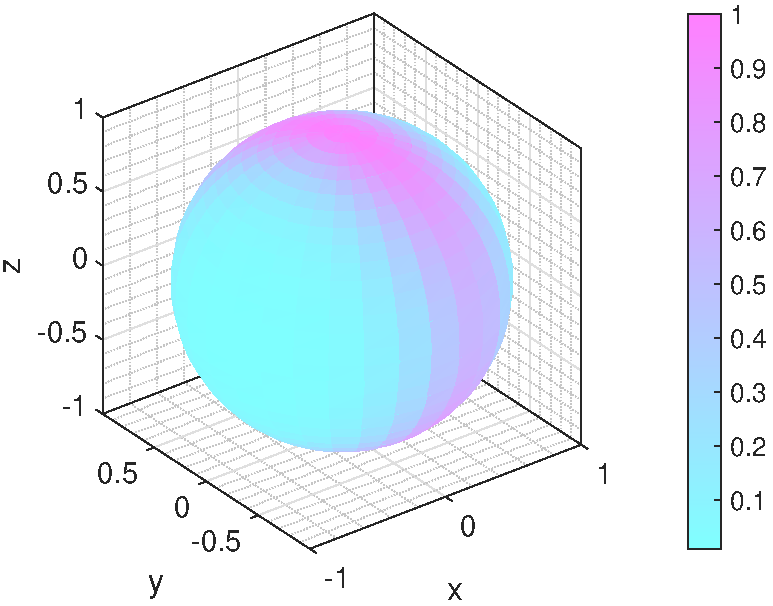
\includegraphics[width=0.21\textwidth]{Definitions/figs/projected_bingham_1}
        \label{fig:bd:project1}
    }
    ~
    \subfigure {
        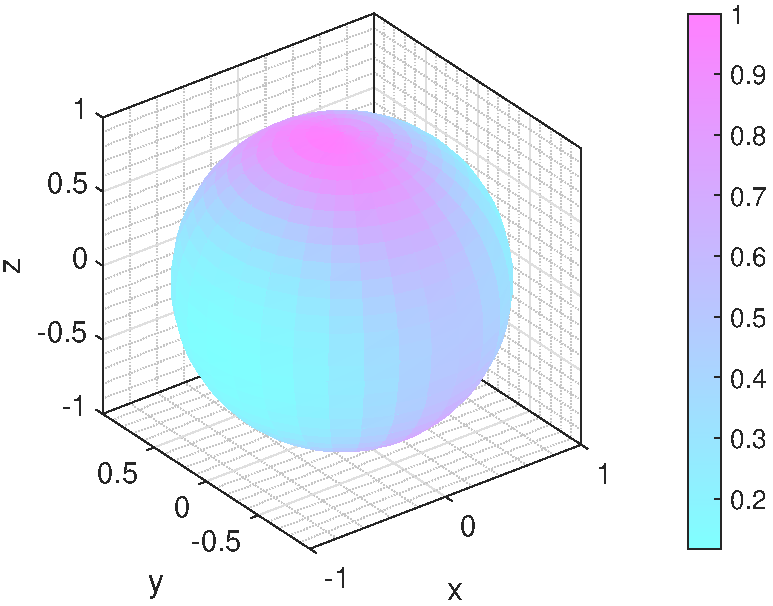
\includegraphics[width=0.21\textwidth]{Definitions/figs/projected_bingham_2}
        \label{fig:bd:project2}
    }
    ~
    \subfigure {
        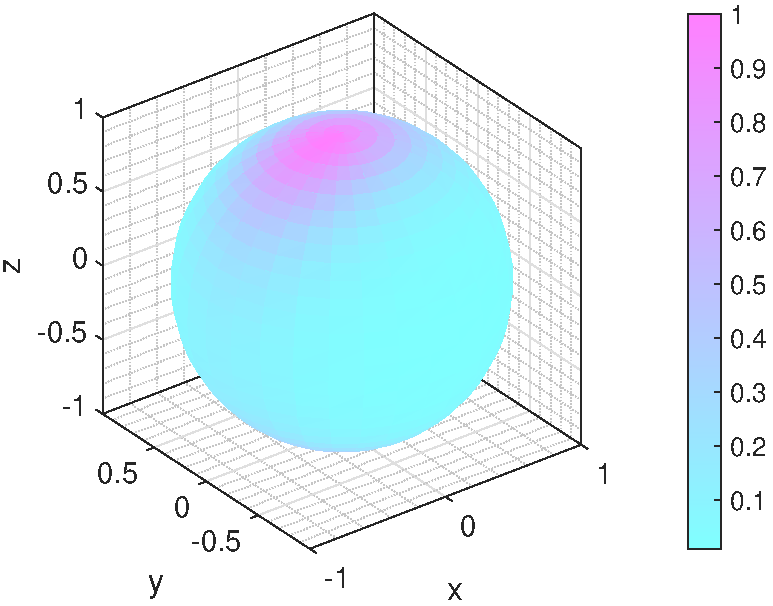
\includegraphics[width=0.21\textwidth]{Definitions/figs/projected_bingham_3}
        \label{fig:bd:project3}
    }
     ~
    \subfigure {
        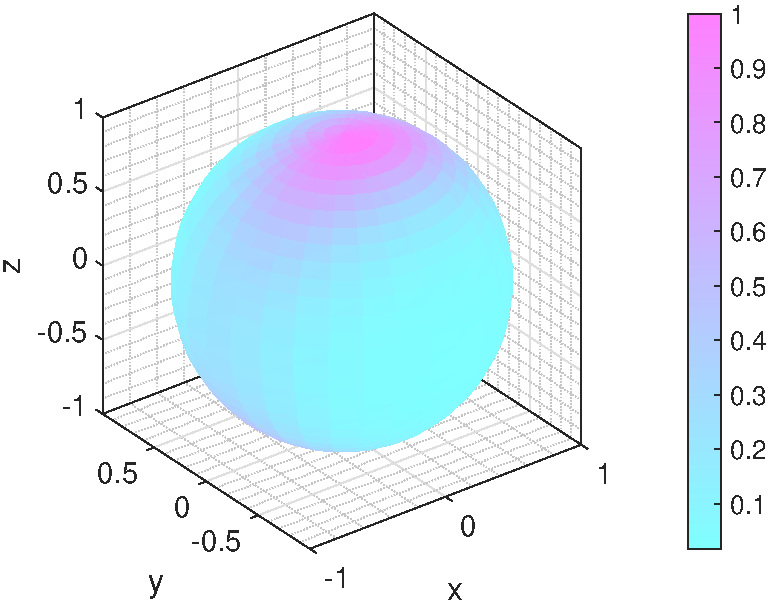
\includegraphics[width=0.21\textwidth]{Definitions/figs/projected_bingham_4}
        \label{fig:bd:project4}
    }
\caption{The probability density function of a unit vector under the marginal distribution of the proposed model, which is projected on hypersphere $S^{3}$ with ${\rm diag}(z)=[-4.72,  -2.15, -0.60]$. The colors encode the value of the probability on the Bingham distribution over the whole sphere.}
    \label{fig:bingham_projected}
\end{figure}  
%%%%%%%%%%%%%%%%%%%%%%%%%%%%%%%%%%%%%%%%%%

%%%%%%%%%%%%%%%%%%%%%%%%%%%%%%%%%%%%%%%%%%%%%%%%%%%%%%%%%%%%%%%%%%%%%%%%%%%%%%%%%%%%

\section{Result} \label{4}

As expected, unit dual quaternions can be used to represent 3D rotation while the dual part is zero. Thus, (\ref{eq:4}) can be extended to a dual form as:

%%%%%%%BEGIN EQUATION%%%%%%%%%%
\begin{equation} \label{eq:12}
\boldsymbol{\widehat{d}_{r}} = [cos({\frac{\theta}{2}}) + sin({\frac{\theta}{2}})(v_1 i + v_2 j + v_3 k)] + \epsilon \cdot 0
\end{equation}
%%%%%%%END EQUATION%%%%%%%%%%%%
where $\boldsymbol{v} = (v_1, v_2, v_3), ||\boldsymbol{v}|| = 1$.

This work utilizes dual quaternions to generate the form of the 3D translation. A vector $\boldsymbol{t} = (t_1,t_2,t_3)^T \in \mathbb{R}^3$ embedded in the skew-field $\mathbb{H}_D$ is represented by the following:
%%%%%%%BEGIN EQUATION%%%%%%%%%%
\begin{equation} \label{eq:13}
    \boldsymbol{\widehat{d}_{t}} = 1 + {\frac{\epsilon}{2}(0 + t_1 i + t_2 j + t_3 k)}
\end{equation}
%%%%%%%END EQUATION%%%%%%%%%%%%
To combine rotations and translations, the product of two unit dual quaternions is used according to ($\ref{eq:6}$). A rotation with a subsequent translation is given as follows:

%%%%%%%BEGIN EQUATION%%%%%%%%%%
\begin{equation} \label{eq:14}
\begin{split}
\boldsymbol{\widehat{d}_{t}} \otimes \boldsymbol{\widehat{d}_{r}} & =[{1+{\frac{\epsilon}{2}}(t_1 i + t_2 j + t_3 k)}] \cdot [{cos({\frac{\theta}{2}}) + \boldsymbol{v}sin({\frac{\theta}{2}})}] \\
& = cos({\frac{\theta}{2}})+sin({\frac{\theta}{2}})(v_1 i + v_2 j + v_3 k)+ {\frac{\epsilon}{2}}{\{} \\
&\quad - sin(\frac{\theta}{2})({v_1}{t_1} + {v_2}{t_2} + {v_3}{t_3}) \\
&\quad + [cos(\frac{\theta}{2})t_1 + sin(\frac{\theta}{2})({v_3}{t_2} - {v_2}{t_3})]i \\
&\quad + [cos(\frac{\theta}{2}){t_2} + sin(\frac{\theta}{2})({v_1}{t_3}-{v_3}{t_1})]j \\
&\quad +[cos(\frac{\theta}{2})t_3 + sin(\frac{\theta}{2})({v_2}t_1  - {v_1}t_2)]k {\}} \\
& =: {d_0} + {d_1}{i} + {d_2}{j} + {d_3}k + {\epsilon}({d_4} + {d_5}i + {d_6}j + {d_7}k)
\end{split} 
\end{equation}
%%%%%%%END EQUATION%%%%%%%%%%
A dual quaterinon in the form of (\ref{eq:14}) is still a unit dual quaternion, and there is no restriction on translation that must be unit-length. According to the defined norm property of the unit dual quaternion, that is, ${p_0}{q_0} + {p_1}{q_1} + {p_2}{q_2}+{p_3}{q_3} = 0$, this property provides ingredients to our algorithm for translation.

According to (\ref{eq:5}), the first four entries are interpreted as the non-dual part, which describes the rotation, and its last four entries are interpreted as a dual part of $\boldsymbol{d}_{\boldsymbol{\widehat{x}}}$. That is:

%%%%%%%BEGIN EQUATION%%%%%%%%%%
\begin{equation} \label{eq:15}
    \boldsymbol{d}_{\boldsymbol{\widehat{x}}} =
    ({d_0},{d_1},{d_2},{d_3},{d_4},{d_5},{d_6},{d_7})^{T}.
\end{equation}
%%%%%%%END EQUATION%%%%%%%%%%

Represented by the vector form, the unit dual quaternion can be written as $\boldsymbol{d}_{\boldsymbol{\widehat{x}}} = \boldsymbol{\widetilde{q}}_{r} + \epsilon \boldsymbol{\widetilde{q}}_{d}$, decomposing into the non-dual part $\boldsymbol{\widetilde{q}}_{r} = ({d_0}, {d_1}, {d_2}, {d_3})$ and the dual part $\boldsymbol{\widetilde{q}}_{d} = ({d_4}, {d_5}, {d_6}, {d_7})$.

Furthermore, the Hamilton operator $(\cdot)^{+} \in \mathbb{R}^{4 \times 4}$ is associated with (\ref{eq:8}), and the translation part can be derived from (\ref{eq:14}) as follows: 

%%%%%%%BEGIN EQUATION%%%%%%%%%%
\begin{equation} \label{eq:16}
\boldsymbol{\widetilde{q}}_{t} = 2 \cdot 
% \boldsymbol{Q}_{q^*_r}^{+}
{\widetilde{\boldsymbol{q}}_{r}^{*+}} \cdot \boldsymbol{\widetilde{q}}_d, 
\end{equation}
%%%%%%%END EQUATION%%%%%%%%%%
where $\widetilde{\boldsymbol{q}}_{r}^{*} = ({q_0}, -\boldsymbol{q}) = ({d_0}, -{d_1},-{d_2}, -{d_3})$ is the conjugate of $\widetilde{\boldsymbol{q}}_{r}$.


{Algorithm ~\ref{algo1}} shows a robust method to generate the rotation angle, axis, and translation in 3D space by sampling from the proposed distribution. Furthermore, this work applies {Algorithm~\ref{algo1}} to several sets of the samples generated from the proposed distribution, and the results are shown in Figure \ref{fig:transformed_samples}.
%%%%%%%%%%%%%%%%%%%%%%%%%%%%%%%%%%%%%%%%%%
\vspace{6pt}%{}

\begin{algorithm}[H]
\DontPrintSemicolon
\KwInput{A sampled %MDPI: Is the font color necessary?. %Lei Zhang: it is necessary, like the coment of the pseudo code.
 random vector $\boldsymbol{w}_{\widehat{\boldsymbol{x}}} = (w_0, \dots, w_7)^{T} \in \mathbb{R}^{8}$}
\tcc{Compute the rotation angle}
${\phi} \leftarrow {2 \cdot \atantwo(\sqrt{{w_1}^2 + {w_2}^2 + {w_3}^2}, w_0)}$ \;
\tcc{Compute the rotational arbitrary vector}
${v_1} \leftarrow {w_1/sin(\phi/2)}$ \;
${v_2} \leftarrow {w_2/sin(\phi/2)}$ \;
${v_3} \leftarrow {w_3/sin(\phi/2)}$ \;
\tcc{Compute the translation}
${t_1} \leftarrow {2 \cdot ({w_0}{w_5} - {w_1}{w_4} + {w_2}{w_7} - {w_3}{w_6}) }$ \;
${t_2} \leftarrow {2 \cdot ({w_0}{w_6} - {w_1}{w_7} - {w_2}{w_4} + {w_3}{w_5}) }$ \;
${t_3} \leftarrow {2 \cdot ({w_0}{w_7} + {w_1}{w_6} - {w_2}{w_5} - {w_3}{w_4})}$ \;

\KwOutput{Rotation angle $\phi$, rotational arbitrary vector $\boldsymbol{v} = (v_1, v_2, v_3)$ and translation vector $\boldsymbol{t} = (t_1, t_2, t_3)$}
\caption{Recover the corresponding translation and rotation from sampled vector on the proposed distribution.} \label{algo1}
\end{algorithm}
%%%%%%%%%%%%%%%%%%%%%%%%%%%%%%%%%%%%%%%%%%

The 6D pose is obtained by the random vector sampled from the proposed distribution. Each sample from our distribution appears in the antipodal symmetry in rotations. Compared with the planar rigid motion case \cite{gilitschenskiNewProbabilityDistribution2014}, our distribution breaks the antipodal symmetry in the translation that $\boldsymbol{t}$ and $-\boldsymbol{t}$ are denoted as positions that always have the same probability values.

%%%%%%%%%%%%%%%%%%%%%%%%%%%%%%%%%%%%%%%%%%
\begin{figure}[H]
\centering
    \centering
    \subfigure {
        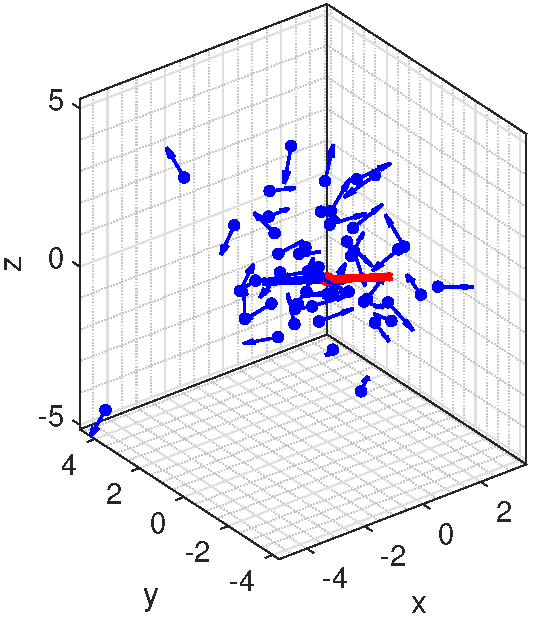
\includegraphics[scale=0.3]{Definitions/figs/c2-se3bingham-pose-50}
        \label{fig:samles:1}
    }
     ~
    \subfigure {
        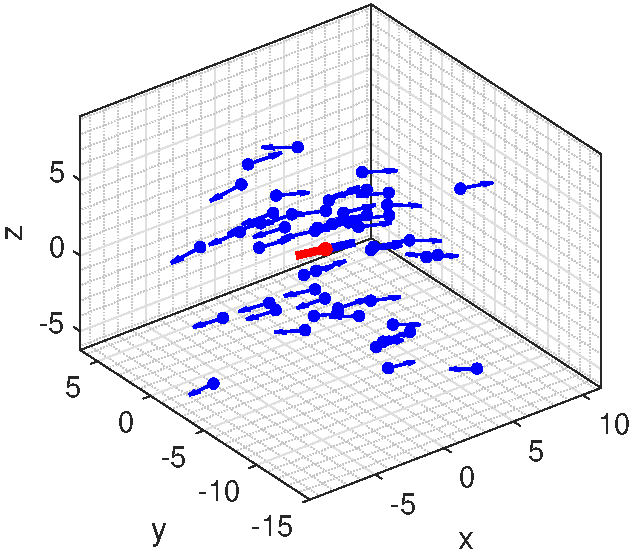
\includegraphics[scale=0.3]{Definitions/figs/c8-se3bingham-pose-50}
        \label{fig:samles:2}
    }
     ~
    \subfigure {
        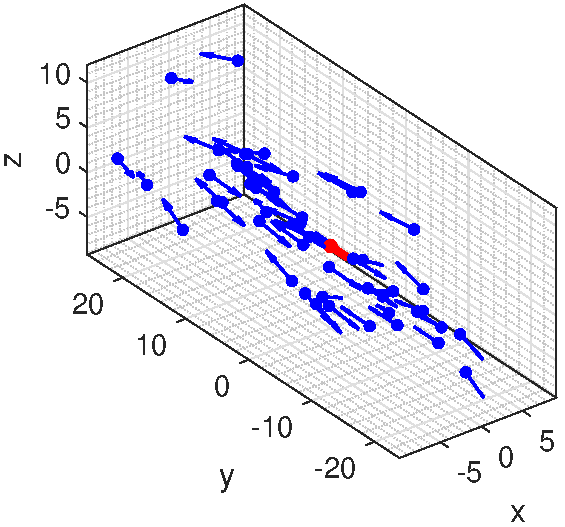
\includegraphics[scale=0.3]{Definitions/figs/c11-se3bingham-pose-50}
        \label{fig:samles:3}
    }
    ~
    \subfigure {
        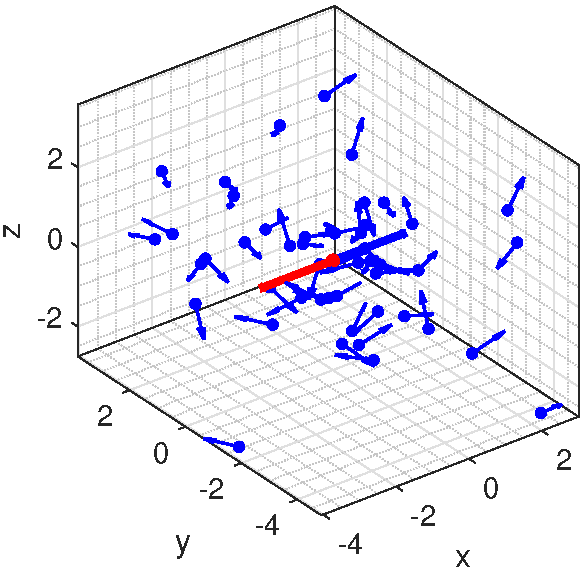
\includegraphics[scale=0.3]{Definitions/figs/c15-se3bingham-pose-50}
        \label{fig:samles:4}
    }
    \\
    ~
    \subfigure {
        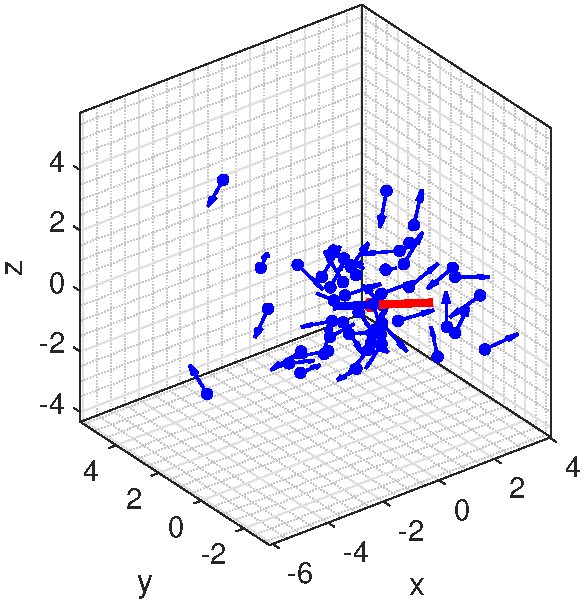
\includegraphics[scale=0.3]{Definitions/figs/c2-se3bingham-pose-50-transformed}
        \label{fig:transformation:1}
    }
    ~
    \subfigure {
        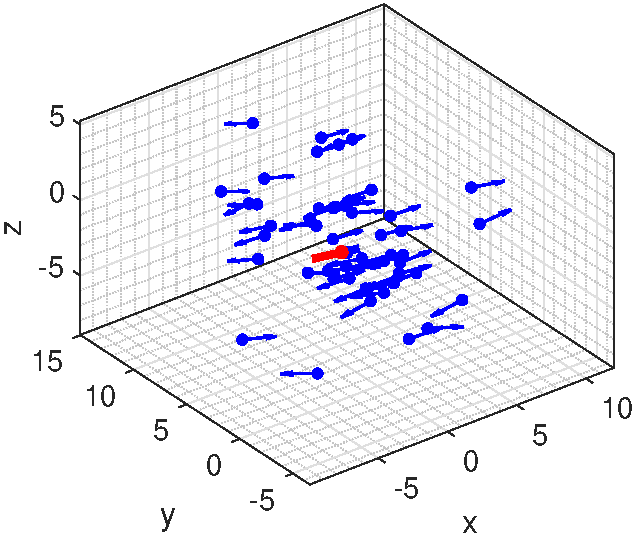
\includegraphics[scale=0.3]{Definitions/figs/c8-se3bingham-pose-50-transformed}
        \label{fig:transformation:2}
    }
    ~
    \subfigure {
        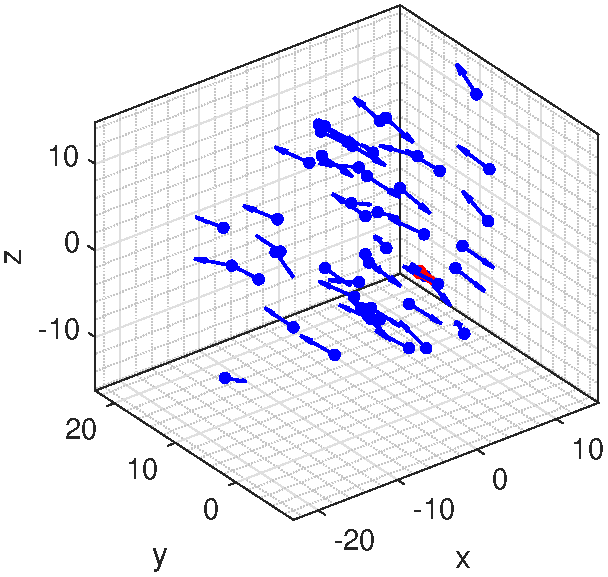
\includegraphics[scale=0.3]{Definitions/figs/c11-se3bingham-pose-50-transformed}
        \label{fig:transformation:3}
    }
    ~
    \subfigure {
        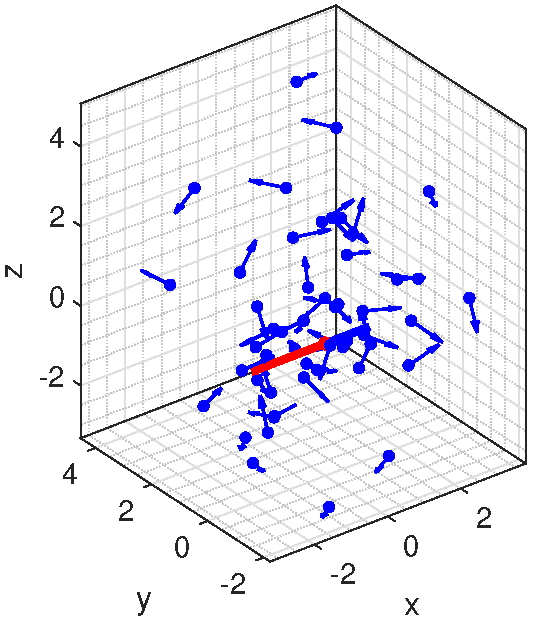
\includegraphics[scale=0.3]{Definitions/figs/c15-se3bingham-pose-50-transformed}
        \label{fig:transformation:4}
    }
\caption{In the first row, the rotation after the translation applies to sets sampled from the proposed distribution, the blue dots mean the position in 3D space, the rotation axis is represented by an arrow. In the bottom row, set the translation after the rotation. The mode in both rows appears as the antipodal symmetry in the representation of rotation; there is no such property in the position that recovers from the proposed distribution ({Zoom in the figure to see the detail}).} \label{fig:transformed_samples}
\end{figure}
%%%%%%%%%%%%%%%%%%%%%%%%%%%%%%%%%%%%%%%%%%

%%%%%%%%%%%%%%%%%%%%%%%%%%%%%%%%%%%%%%%%%%%%%%%%%%%%%%%%%%%%%%%%%%%%%%%%%%%%%%%%%%%%

\section{Conclusions} \label{5}
This work proposes a distribution over the 6D pose in order to capture the uncertainty which is typically ignored by the pose estimation task. Our model takes the periodic nature of the underline structure into consideration, such as antipodal symmetry, which is suitable for high-noise regimes. The proposed distribution eliminates the drawbacks from initializing the $SE(2)$, in which the position is ambiguous due to antipodal symmetry, and our distribution setting is closer to reality.

However, we assume that the Gaussian on the correlation part leads to a better, but still imperfect, answer. Many beautiful properties in the parameter matrix of the proposed distribution have not been explored. {Still, a unified distribution exists to couple the rotation and translation.}

In the future, we will verify the proposed distribution in practical applications, such point cloud registration, as well as the most important one, the 6D pose estimation task.  {Last but not least, the combination of {the neural network} with the proposed probability to regress the object pose is worth endeavoring.}

%%%%%%%%%%%%%%%%%%%%%%%%%%%%%%%%%%%%%%%%%%%%%%%%%%%%%%%%%%%%%%%%%%%%%%%%%%%%%%%%%%%%%%%%%%%%%%%%%
\vspace{6pt} 

\authorcontributions{{Conceptualization, L.Z.; methodology, L.Z.; software,  L.Z.; validation,  L.Z.; formal analysis,  L.Z. and Y.L.; investigation,  L.Z.; mathematical deduction,  L.Z.; data curation, L.Z.; writing---original draft preparation,  L.Z.; writing---review and editing,  L.Z. and Y.L.; visualization, L.Z.; supervision, H.S. and Y.L.; project administration, H.S. and Y.L. All authors have read and agreed to the published version of the manuscript.}}


\funding{{This research received no external funding.}} %Lei Zhang: No funding

\acknowledgments{Appreciations to Srivatsan and Gilitschenski. They introduced the work to me. Thanks to Qiushu Chen for helping check the manuscript, and Zhenhui Tang and Zhengxiao Zhao, etc. involved in the discussion. Thanks to the open-source code from ISAS Lab at KTI and Kurz's simulation software, I have a comprehensive understanding of the Bingham distribution.}

\institutionalreview{Not applicable.}

\informedconsent{Not applicable.}

\dataavailability{{Data sharing is not applicable to this article.}}

\conflictsofinterest{The authors declare no conflict of interest.} 

%%%%%%%%%%%%%%%%%%%%%%%%%%%%%%%%%%%%%%%%%%%%%%%%%%%%%%%%%%%%%%%%%%%%%%%%%%%%%%%%%%%%
%% Optional
\appendixtitles{yes} % Leave argument "no" if all appendix headings stay EMPTY (then no dot is printed after "Appendix A"). If the appendix sections contain a heading then change the argument to "".
\appendixstart
\appendix
\section[\appendixname~\thesection]{Proof of Lemma 3}\label{append1}

The parameter matrix C in the distribution can be rewritten as the UDL form by \textit{Schur Complement}:

%%%%%%%BEGIN EQUATION%%%%%%%%%%
\begin{align*}
{{\begin{pmatrix}\boldsymbol{x}_{r} \\ \boldsymbol{x}_{d}\end{pmatrix}}^T} & {\begin{pmatrix}\boldsymbol{C}_{11} & \boldsymbol{C}_{12} \\ \boldsymbol{C}_{21} & \boldsymbol{C}_{22} \end{pmatrix}} {\begin{pmatrix} \boldsymbol{x}_{r} \\ \boldsymbol{x}_{d} \end{pmatrix}} \\ 
= {\begin{pmatrix}\boldsymbol{C}_{r} \\ \boldsymbol{x}_{d}\end{pmatrix}}^T & \begin{pmatrix} 1 & \boldsymbol{C}_{12}\boldsymbol{C}_{22}^{-1} \\ 0 & 1 \end{pmatrix}{\begin{pmatrix} \boldsymbol{C}_{11} - \boldsymbol{C}_{12}\boldsymbol{C}_{22}^{-1}\boldsymbol{C}_{21} & 0 \\ 0 & \boldsymbol{C}_{22}\end{pmatrix}} %\\ &
{\begin{pmatrix} 1 & 0 \\ \boldsymbol{C}_{22}^{-1}\boldsymbol{C}_{21} & \end{pmatrix}}{\begin{pmatrix}\boldsymbol{x}_{r}\\\boldsymbol{x}_{d}\end{pmatrix}} \\ &
= \boldsymbol{x}_{r}^T \left({\boldsymbol{C}_{11}}-{\boldsymbol{C}_{12}}{\boldsymbol{C}_{22}^{-1}\boldsymbol{C}_{21}}\right)\boldsymbol{x}_{r} + % \\ &
\left(\boldsymbol{x}_{d} + {\boldsymbol{C}_{22}}^{-1}{\boldsymbol{C}_{21}}{x}_{r}\right)^{T} {\boldsymbol{C}_{22}}\left(\boldsymbol{x}_{d}+{\boldsymbol{C}_{22}}^{-1}{\boldsymbol{C}_{21}}\boldsymbol{x}_{r}\right)
\end{align*}
%%%%%%%END EQUATION%%%%%%%%%%
where, once again, $\boldsymbol{A}_{1} = \boldsymbol{C}_{11} - \boldsymbol{C}_{12}\boldsymbol{C}_{22}^{-1} \boldsymbol{C}_{21}$, $\boldsymbol{A}_{2} = -\boldsymbol{C}_{22}^{-1}\boldsymbol{C}_{21}$.


%%%%%%%%%%%%%%%%%%%%%%%%%%%%%%%%%%%%%%%%%%%%%%%%%%%%%%%%%%%%%%%%%%%%%%%%%%%%%%%%%%%%

\begin{adjustwidth}{-\extralength}{0cm}
%\centering %% If there is a figure in wide page, please release command \centering
\reftitle{References}

\begin{thebibliography}{999}
%Lei Zhang: format each bibtem and highlight the changes I updated.
%%%%%%%%%% 1 %%%%%%%%%% 
\bibitem[Qidan \em{et~al.}(2017) Qidan, Hongle, Chengtao, and Peng]{qidan2017rapid}
Qidan, Z.; Hongle, X.; Chengtao, C.; Peng, L.
\newblock A rapid and precise self-localization approach of mobile robot based on binocular omni-directional vision.
\newblock In Proceedings of the  2017 36th Chinese Control Conference (CCC), {Dalian, China, 26-28 July} 2017; pp. 6835--6840.
%MDPI: Please add the location (city and country) and date rang (day month year) for the conference. Similar highlights are same meaning

%%%%%%%%%% 2 %%%%%%%%%% 
\bibitem[Barfoot(2017)]{barfootStateEstimationRobotics2021}
Barfoot, T.D.
\newblock {\em State Estimation for Robotics}; Cambridge University Press: Cambridge, UK, 2017.

%%%%%%%%%% 3 %%%%%%%%%% 
\bibitem[Zeng~{\textit{et al.}}(2018)]{zengRoboticPickandPlaceNovel2018}
 {{Zeng, A., Song, S., Yu, K.T., Donlon, E., Hogan, F.R., Bauza, M., Ma, D., Taylor, O., Liu, M., Romo, E.}}  %MDPI: Please include the first ten authors' names before using et al. in references %Lei Zhang: top 10.
\newblock Robotic Pick-and-Place of Novel Objects in Clutter with Multi-Affordance Grasping and Cross-Domain Image Matching.
\newblock In Proceedings of the 2018 IEEE International Conference on Robotics and Automation (ICRA), {Brisbane, Australia, 21-25 May} 2018; pp. 3750--3757,
\newblock
doi:{\changeurlcolor{black}\href{https://doi.org/10.1109/ICRA.2018.8461044}{\detokenize{10.1109/ICRA.2018.8461044}}}.

%%%%%%%%%% 4 %%%%%%%%%% 
\bibitem[Krizhevsky \em{et~al.}(2012)Krizhevsky, Sutskever, and Hinton]{krizhevsky2012imagenet}
Krizhevsky, A.; Sutskever, I.; Hinton, G.E.
\newblock Imagenet classification with deep convolutional neural networks.
\newblock {\em Adv. Neural Inf. Process. Syst.} {\bf 2012}, {\em 25}, {pp. 1097--1105}.

%%%%%%%%%% 5 %%%%%%%%%% 
\bibitem[Deng \em{et~al.}(2009)Deng, Dong, Socher, Li, Li, and Fei-Fei]{deng2009imagenet}
Deng, J.; Dong, W.; Socher, R.; Li, L.J.; Li, K.; Fei-Fei, L.
\newblock Imagenet: A large-scale hierarchical image database.
\newblock In Proceedings of the  2009 IEEE Conference on Computer Vision and Pattern Recognition {(CVPR), Miami, Florida, 20-25 June 2009;} pp. 248--255.

%%%%%%%%%% 6 %%%%%%%%%% 
\bibitem[Shamsfakhr and Bigham(2020)]{shamsfakhr2020gsr}
Shamsfakhr, F.; Bigham, B.S.
\newblock GSR: Geometrical scan registration algorithm for robust and fast robot pose estimation.
\newblock {\em Assem. Autom.} {{\bf 2020}, {\em {40}}, {pp. 801--817}}. %MDPI: Please add volume number and page number, or doi. Similar highlights are same meaning

%%%%%%%%%% 7 %%%%%%%%%% 
\bibitem[Okorn \em{et~al.}(2020)Okorn, Xu, Hebert, and Held]{okornLearningOrientationDistributions2020}
Okorn, B.; Xu, M.; Hebert, M.; Held, D.
\newblock Learning Orientation Distributions for Object Pose Estimation.
\newblock In Proceedings of the 2020 IEEE/RSJ International Conference on Intelligent Robots and Systems (IROS), {Las Vegas,USA, 25-29 January 2020;} pp. 10580--10587, %Lei Zhang: but the conference delayed by the COVID-19, https://www.iros2020.org/
\newblock
doi:{\changeurlcolor{black}\href{https://doi.org/10.1109/IROS45743.2020.9340860}{\detokenize{10.1109/IROS45743.2020.9340860}}}.

%%%%%%%%%% 8 %%%%%%%%%% 
\bibitem[Xiang \em{et~al.}(2018)Xiang, Schmidt, Narayanan, and Fox]{xiangPoseCNNConvolutionalNeural2018}
Xiang, Y.; Schmidt, T.; Narayanan, V.; Fox, D.
\newblock PoseCNN: A Convolutional Neural Network for 6D Object Pose Estimation in Cluttered Scenes.
\newblock {Proceedings of robotics: Science and systems (RSS), Pittsburgh, Pennsylvania, USA,} {26-30 June} {\bf {2018}}; %http://www.roboticsproceedings.org/rss14/p19.html
\newblock
doi:{\changeurlcolor{black}\href{https://doi.org/10.15607/RSS.2018.XIV.019}{\detokenize{10.15607/RSS.2018.XIV.019}}}. %Lei Zhang: I combine the doi from 10.15607/RSS.2018.XIV.019 like yours, there is no exact pages for this citation.

%%%%%%%%%% 9 %%%%%%%%%% 
\bibitem[Wang \em{et~al.}(2019)Wang, Xu, Zhu, Martín-Martín, Lu, Fei-Fei, and Savarese]{wangDenseFusion6DObject2019}
Wang, C.; Xu, D.; Zhu, Y.; Martín-Martín, R.; Lu, C.; Fei-Fei, L.; Savarese, S.
\newblock DenseFusion: 6D Object Pose Estimation by Iterative Dense Fusion.
\newblock In Proceedings of the  2019 IEEE/CVF Conference on Computer Vision and Pattern Recognition (CVPR), {Long Beach, CA, USA, 16-20 June 2019;} pp. 3338--3347,
\newblock
doi:{\changeurlcolor{black}\href{https://doi.org/10.1109/CVPR.2019.00346}{\detokenize{10.1109/CVPR.2019.00346}}}.

%%%%%%%%%% 10 %%%%%%%%%% 
\bibitem[Hodaň \em{et~al.}(2020)Hodaň, Baráth, and Matas]{hodanEPOSEstimating6D2020}
Hodaň, T.; Baráth, D.; Matas, J.
\newblock {{EPOS}}: {{Estimating 6D Pose}} of {{Objects With Symmetries}}.
\newblock In Proceedings of the  2020 IEEE/CVF Conference on Computer Vision and Pattern Recognition {(CVPR), Virtual, 14-19 June 2020;} pp. 11700--11709,
\newblock
doi:{\changeurlcolor{black}\href{https://doi.org/10.1109/CVPR42600.2020.01172}{\detokenize{10.1109/CVPR42600.2020.01172}}}. %Lei Zhang: I check from https://cvpr2020.thecvf.com/, gives the virtual

%%%%%%%%%% 11 %%%%%%%%%% 
\bibitem[Manhardt~{\textit{ et al.}}(2019)]{manhardtExplainingAmbiguityObject2019}
{Manhardt, F., Arroyo, D.M., Rupprecht, C., Busam, B., Birdal, T., Navab, N. and Tombari, F.}
\newblock Explaining the Ambiguity of Object Detection and 6D Pose From Visual Data.
\newblock In Proceedings of the  2019 IEEE/CVF International Conference on Computer Vision {(ICCV), Seoul, Korea, 27 October-2 November 2019;} pp. 6840--6849,
\newblock
doi:{\changeurlcolor{black}\href{https://doi.org/10.1109/ICCV.2019.00694}{\detokenize{10.1109/ICCV.2019.00694}}}.

%%%%%%%%%% 12 %%%%%%%%%% 
\bibitem[Deng \em{et~al.}(2019)Deng, Mousavian, Xiang, Xia, Bretl, and Fox]{dengPoseRBPFRaoBlackwellizedParticle2019}
Deng, X.; Mousavian, A.; Xiang, Y.; Xia, F.; Bretl, T.; Fox, D.
\newblock PoseRBPF: A Rao-Blackwellized Particle Filter for 6D Object Pose Tracking.
\newblock  {Proceedings of Robotics: Science and Systems}, {FreiburgimBreisgau, Germany, 22-26 June} \textbf{{2019}};
\newblock
doi:{\changeurlcolor{black}\href{https://doi.org/10.15607/RSS.2019.XV.049}{\detokenize{10.15607/RSS.2019.XV.049}}}.

%%%%%%%%%% 13 %%%%%%%%%% 
\bibitem[Horn \em{et~al.}(1988)Horn, Hilden, and Negahdaripour]{hornClosedformSolutionAbsolute1987}
Horn, B.; Hilden, H.; Negahdaripour, S.
\newblock Closed-Form Solution of Absolute Orientation using Orthonormal Matrices.
\newblock {\em J. Opt. Soc. Am. A} {\bf 1988}, {\em 5},~1127--1135,
\newblock
doi:{\changeurlcolor{black}\href{https://doi.org/10.1364/JOSAA.5.001127}{\detokenize{10.1364/JOSAA.5.001127}}}.

%%%%%%%%%% 14 %%%%%%%%%% 
\bibitem[Prokudin \em{et~al.}(2018)Prokudin, Gehler, and Nowozin]{prokudinDeepDirectionalStatistics2018}
Prokudin, S.; Gehler, P.; Nowozin, S.
\newblock Deep Directional Statistics: Pose Estimation with Uncertainty Quantification.
\newblock In Proceedings of the  2018 European Conference on Computer Vision {(ECCV), Munich, Germany, 8-14 September 2018;} pp. 534--551.
\newblock
doi:{\changeurlcolor{black}\href{https://doi.org/10.1007/978-3-030-01240-3_33}{\detokenize{10.1007/978-3-030-01240-3_33}}}.
%Lei Zhang: added doi

%%%%%%%%%% 15 %%%%%%%%%% 
\bibitem[Daniilidis(1999)]{daniilidisHandEyeCalibrationUsing1999}
Daniilidis, K.
\newblock Hand-{{Eye Calibration Using Dual Quaternions}}.
\newblock {\em  Int. J. Robot. Res.} {\bf 1999}, {\em 18},~286--298.

%%%%%%%%%% 16 %%%%%%%%%% 
\bibitem[Goddard and Abidi(1998)]{goddardPoseMotionEstimation1998} Goddard, J.S.; Abidi, M.A.
\newblock Pose and Motion Estimation Using Dual Quaternion-Based Extended Kalman Filtering.
\newblock In \emph{Three-Dimensional Image Capture and Applications}; Ellson, R.N.,
Nurre, J.H., Eds.; International Society for Optics and Photonics, {SPIE: Bellingham, WA, USA,} {\bf 1998}; pp. 189--200,
%MDPI: Please add the location of the publisher. %Lei Zhang: actually, I am not sure it is correct. Event: Photonics West '98 Electronic Imaging, 1998, San Jose, CA, United States https://www.spiedigitallibrary.org/conference-proceedings-of-spie/3313/0000/Pose-and-motion-estimation-using-dual-quaternion-based-extended-Kalman/10.1117/12.302453.short?SSO=1
 
\newblock
doi:{\changeurlcolor{black}\href{https://doi.org/10.1117/12.302453}{\detokenize{10.1117/12.302453}}}.

%Lei Zhang: removed from introduction
% \bibitem[Besl and McKay(1992)]{beslMethodRegistration3D1992}
% Besl, P.; McKay, N.D.
% \newblock A Method for Registration of 3-D Shapes.
% \newblock {\em IEEE Trans. Pattern Anal. Mach. Intell.} {\bf 1992}, {\em 14},~239--256.

%%%%%%%%%% 17 %%%%%%%%%% 
\bibitem[Lin \em{et~al.}(2021)Lin, Liang, and Chen]{linRoboticGraspingMultiView2021}
Lin, H.Y.; Liang, S.C.; Chen, Y.K.
\newblock Robotic Grasping with Multi-View Image Acquisition and Model-Based Pose Estimation.
\newblock {\em IEEE Sens. J.} {\bf 2021}, {\em 21},~11870--11878.

%%%%%%%%%% 18 %%%%%%%%%% 
\bibitem[Srivatsan \em{et~al.}(2018)Srivatsan, Xu, Zevallos, and Choset]{arun2018probabilistic}
Srivatsan, R.A.; Xu, M.; Zevallos, N.; Choset, H.
\newblock Probabilistic pose estimation using a Bingham distribution-based linear filter.
\newblock {\em  Int. J. Robot. Res.} {\bf 2018}, {\em 37},~1610--1631,
\newblock
doi:{\changeurlcolor{black}\href{https://doi.org/10.1177/0278364918778353}{\detokenize{10.1177/0278364918778353}}}.

%%%%%%%%%% 19 %%%%%%%%%% 
\bibitem[Li \em{et~al.}(2019)Li, Pfaff, and Hanebeck]{liGeometryDrivenStochasticModeling2019}
Li, K.; Pfaff, F.; Hanebeck, U.D.
\newblock Geometry-Driven Stochastic Modeling of {{SE}}(3) States Based on Dual Quaternion Representation.
\newblock In Proceedings of the 2019 IEEE International Conference on Industrial Cyber Physical Systems {(ICPS), Taipei, Taiwan, 6-9 May 2019;} pp. 254--260,
\newblock
doi:{\changeurlcolor{black}\href{https://doi.org/10.1109/ICPHYS.2019.8780254}{\detokenize{10.1109/ICPHYS.2019.8780254}}}.
%Lei Zhang: https://ieeexplore.ieee.org/abstract/document/8780254/

%%%%%%%%%% 20 %%%%%%%%%% 
\bibitem[Glover and Popovic(2013)]{gloverBinghamProcrusteanAlignment2013}
Glover, J.; Popovic, S.
\newblock Bingham Procrustean Alignment for Object Detection in Clutter.
\newblock In Proceedings of the  2013 IEEE/RSJ International Conference on Intelligent Robots and {Systems, Tokyo, Japan, 3-7 November 2013;} pp. 2158--2165,
\newblock
doi:{\changeurlcolor{black}\href{https://doi.org/10.1109/IROS.2013.6696658}{\detokenize{10.1109/IROS.2013.6696658}}}.

%%%%%%%%%% 21 %%%%%%%%%% 
\bibitem[Gilitschenski \em{et~al.}(2014)Gilitschenski, Kurz, Julier, and Hanebeck]{gilitschenskiNewProbabilityDistribution2014}
Gilitschenski, I.; Kurz, G.; Julier, S.J.; Hanebeck, U.D.
\newblock A New Probability Distribution for Simultaneous Representation of Uncertain Position and Orientation.
\newblock In Proceedings of the 17th International Conference on Information Fusion {(FUSION), Salamanca, Spain, 7-10 July 2014;} pp. 1--7.

%%%%%%%%%% 22 %%%%%%%%%% 
\bibitem[Corke(2017)]{corkeRoboticsVisionControl2017} Corke, P.
\newblock {\em Robotics, {{Vision}} and {{Control}}}; Springer {{Tracts}} in {{Advanced Robotics}}; {Springer International Publishing}: Cham, Switzerland,  2017; Volume 118, p.~45,
\newblock
doi:{\changeurlcolor{black}\href{https://doi.org/10.1007/978-3-319-54413-7}{\detokenize{10.1007/978-3-319-54413-7}}}.

%%%%%%%%%% 23 %%%%%%%%%% 
\bibitem[Jackson \em{et~al.}(2021)Jackson, Tracy, and Manchester]{jacksonPlanningAttitude2021} Jackson, B.E.; Tracy, K.; Manchester, Z.
\newblock Planning with Attitude.
\newblock {\em IEEE Robot. Autom. Lett.} {\bf 2021}, {\em 6}, {pp. 5658-5664},
\newblock
doi:{\changeurlcolor{black}\href{https://doi.org/10.1109/LRA.2021.3052431}{\detokenize{10.1109/LRA.2021.3052431}}}.

%%%%%%%%%% 24 %%%%%%%%%% 
\bibitem[Feiten \em{et~al.}(2009)Feiten, Atwal, Eidenberger, and Grundmann]{feiten20096d}
Feiten, W.; Atwal, P.; Eidenberger, R.; Grundmann, T.
\newblock \emph{{6D Pose Uncertainty} in {Robotic Perception}};
\newblock  Advances in Robotics Research; Springer: Cham, Switzerland, 2009; pp. 89--98,
\newblock
doi:{\changeurlcolor{black}\href{https://doi.org/10.1007/978-3-642-01213-6_9}{\detokenize{10.1007/978-3-642-01213-6_9}}}.

%%%%%%%%%% 25 %%%%%%%%%% 
\bibitem[Stuelpnagel(1964)]{stuelpnagelParametrizationThreeDimensionalRotation1964}
Stuelpnagel, J.
\newblock On the {{Parametrization}} of the {{Three-Dimensional Rotation Group}}.
\newblock {\em SIAM Rev.} {\bf 1964}, {\em 6},~422--430.

%%%%%%%%%% 26 %%%%%%%%%% 
\bibitem[Feiten \em{et~al.}(2013)Feiten, Lang, and Hirche]{feitenRigidMotionEstimation2013}
Feiten, W.; Lang, M.; Hirche, S.
\newblock Rigid Motion Estimation Using Mixtures of Projected {{Gaussians}}.
\newblock In Proceedings of the 16th International Conference on Information Fusion {(FUSION), Istanbul, Turkey, 9-12 July 2013;} pp. 1465--1472.

%%%%%%%%%% 27 %%%%%%%%%% 
\bibitem[Kenwright(2012)]{kenwrightBeginnersGuideDualquaternions2012} Kenwright, B.
\newblock \emph{A Beginners Guide to Dual-Quaternions: What They Are, How They Work, and How to Use Them for {{3D}} Character Hierarchies}; 
\newblock The 20th International Conference on Computer Graphics, Visualization and Computer Vision, WSCG 2012 Communication Proceedings,
{Pilsen, Czech Republic, 25-28 June 2012; pp. 1--13} %MDPI: Please add the publisher and location.

%%%%%%%%%% 28 %%%%%%%%%% 
\bibitem[Kavan \em{et~al.}(2007)Kavan, Collins, {\v Z}{\'a}ra, and O'Sullivan]{kavanSkinningDualQuaternions2007} Kavan, L.; Collins, S.; {\v Z}{\'a}ra, J.; O'Sullivan, C.
\newblock Skinning with Dual Quaternions.
\newblock {I3D '07: Proceedings of the 2007 Symposium on Interactive 3D Graphics and Games}; {ACM Press: New York, NY, USA} %MDPI: Please add the location of the publisher. %Lei Zhang: https://dl.acm.org/doi/proceedings/10.1145/1230100
2007; p.~39.

%%%%%%%%%% 29 %%%%%%%%%% 
\bibitem[Fan \em{et~al.}(2017)Fan, Weng, and  Murphey]{fanDecentralizedRecursiveIdentification2017}
Fan, T.; Weng, H.; Murphey, T.
\newblock Decentralized and Recursive Identification for Cooperative Manipulation of Unknown Rigid Body with Local Measurements.
\newblock In Proceedings of the  2017 IEEE 56th Annual Conference on Decision and Control {(CDC), Melbourne, Australia, 12-15 December 2017;} pp. 2842--2849,
\newblock
doi:{\changeurlcolor{black}\href{https://doi.org/10.1109/CDC.2017.8264073}{\detokenize{10.1109/CDC.2017.8264073}}}.

%%%%%%%%%% 30 %%%%%%%%%% 
\bibitem[Akyar(2008)]{akyarDualQuaternionsSpatial2008}
Akyar, B.
\newblock Dual {{Quaternions}} in {{Spatial Kinematics}} in an {{Algebraic Sense}}.
\newblock {\em Turk. J. Math.} {\bf 2008}, {\em 32},~373--391.

%%%%%%%%%% 31 %%%%%%%%%% 
\bibitem[Bingham(1974)]{binghamAntipodallySymmetricDistribution1974}
Bingham, C.
\newblock An {{Antipodally Symmetric Distribution}} on the {{Sphere}}.
\newblock {\em Ann. Stat.} {\bf 1974}, {\em 2},~1201--1225.
\newblock
doi:{\changeurlcolor{black}\href{https://doi.org/10.1214/aos/1176342874}{\detokenize{10.1214/aos/1176342874}}}.

%%%%%%%%%% 32 %%%%%%%%%% 
\bibitem[Antone(2001)]{antoneRobustCameraPose2001}
Antone, M.E.
\newblock Robust {{Camera Pose Recovery Using Stochastic Geometry}}.
\newblock Ph.D. Thesis,  {Massachusetts Institute of Technology, Cambridge, MA, USA, 2001.} %MDPI: Please add the university and location.

%%%%%%%%%% 33 %%%%%%%%%% 
\bibitem[Kurz \em{et~al.}(2013)Kurz, Gilitschenski, Julier, and Hanebeck]{kurzRecursiveEstimationOrientation2013}
Kurz, G.; Gilitschenski, I.; Julier, S.; Hanebeck, U.D.
\newblock Recursive Estimation of Orientation Based on the {{Bingham}} Distribution.
\newblock In Proceedings of the  16th International Conference on Information Fusion, {(FUSION), Istanbul, Turkey, 9-12 July, 2013;}  pp. 1487--1494.

%%%%%%%%%% 34 %%%%%%%%%% 
\bibitem[Glover \em{et~al.}(2012)Glover, Bradski, Rusu, and Park]{gloverMonteCarloPose2011}
Glover, J.; Bradski, G.; Rusu, R.B.; Park, M.
\newblock Monte {{Carlo Pose Estimation}} with {{Quaternion Kernels}} and the {{Bingham Distribution}}.
\newblock  \emph{Robot. Sci. Syst.}  \textbf{2012}, \emph{7}, 97.

%%%%%%%%%% 35 %%%%%%%%%%
\bibitem[Gilitschenski \em{et~al.}(2020)Gilitschenski, Sahoo, Schwarting, Amini, Karaman, and Rus]{gilitschenskiDEEPORIENTATIONUNCERTAINTY2020}
Gilitschenski, I.; Sahoo, R.; Schwarting, W.; Amini, A.; Karaman, S.; Rus, D.
\newblock Deep Orientation Uncertainty Learning based on a Bingham Loss.
\newblock In Proceedings of the  International Conference on Learning {Representations (ICLR), Addis Ababa, Ethiopia, 25 September 2019}.

%%%%%%%%%% 36 %%%%%%%%%%
\bibitem[Kurz \em{et~al.}(2019)Kurz, Gilitschenski, Pfaff, Drude, Hanebeck, Haeb-Umbach, and Siegwart]{kurzDirectionalStatisticsFiltering2017}
Kurz, G.; Gilitschenski, I.; Pfaff, F.; Drude, L.; Hanebeck, U.D.; Haeb-Umbach, R.; Siegwart, R.Y.
\newblock Directional {{Statistics}} and {{Filtering Using libDirectional}}.
\newblock {\em J. Stat. Softw. Artic.} {\bf 2019}, {\em  89},~1--31,
\newblock
doi:{\changeurlcolor{black}\href{https://doi.org/10.18637/jss.v089.i04}{\detokenize{10.18637/jss.v089.i04}}}.

%%%%%%%%%% 37 %%%%%%%%%%
\bibitem[Anderson(2003)]{andersonIntroductionMultivariateStatistical2003}
Anderson, T.W.
\newblock {\em An Introduction to Multivariate Statistical Analysis}; {Wiley-Interscience}: Hoboken, NJ, USA,  2003.

%%%%%%%%%% 38 %%%%%%%%%%
\bibitem[Kurz \em{et~al.}(2014)Kurz, Gilitschenski, Julier, and  Hanebeck]{kurzRecursiveBinghamFilter2014}
Kurz, G.; Gilitschenski, I.; Julier, S.; Hanebeck, U.
\newblock Recursive {{Bingham Filter}} for {{Directional Estimation Involving}} 180 {{Degree Symmetry}}.
\newblock {\em J. Adv. Inf. Fusion} {\bf 2014}, {\em 9},~90--105.

\end{thebibliography}

\end{adjustwidth}
%%%%%%%%%%%%%%%%%%%%%%%%%%%%%%%%%%%%%%%%%%%%%%%%%%%%%%%%%%%%%%%%%%%%%%%%%%%%%%%%%%%%

\end{document}

